\chapter{抽样分布与估计误差}
\label{chap:sampling-errors}

第~\ref{chap:sample-estimation}章从一组观测出发构造了估计：用样本比例估计不合格率，用样本均值估计测量均值，用修正样本方差估计波动大小。
设想我们随机检查了$80$件产品，发现$24$件不合格，于是报告不合格率约为$0.3$。
这个数字离真实不合格率有多远？如果明天换一批$80$件重新检查，报告会变成多少？
再检查$800$件，误差会缩小到什么程度？这些问题都不针对已经算出的那个数，而针对“按同一规则重复抽样、重复计算”时结果的波动。

本章先确定误差的含义。
同一个计算规则在不同样本上给出不同结果，所以统计量本身也有分布；
它的标准差、它的平均位置与目标的距离，以及它到目标的平均平方距离，分别回答“波动多大”“是否系统偏离”“总体上离得多远”。
有了这些指标，我们再研究三类能够说明误差大小的依据。

第一类依据是精确分布：如果总体服从正态分布，样本均值、样本方差及它们的比值都有可以写出的分布，这就是卡方分布、$t$分布与$F$分布的来源。
第二类依据是有限样本概率界：只知道均值或方差时，Markov与Chebyshev不等式仍能对任意固定的样本量给出误差超过阈值的概率上界。
第三类依据是极限定理：样本量增大时，大数定律说明样本均值靠近总体均值，中心极限定理进一步描述放大后的误差近似服从正态分布。
三类依据的条件与结论各不相同，第~\ref{chap:intervals-tests-prediction}章构造区间、检验与预测时会分别用到它们。

\section{抽样分布与误差指标}
\label{sec:samp-errors}

本节固定总体与样本量，把“重复抽样”这个想象中的操作落实成统计量的分布，再用它定义标准误、偏差与均方误差。
这些指标描述的是计算规则的表现，而不是某一次估计值的对错。

\subsection{统计量的抽样分布}

\paragraph{重复抽样下的样本比例}
回到产品检查。设每件产品不合格的概率为$p$，各件是否不合格相互独立，第$i$件的结果记为$X_i\sim\operatorname{Bernoulli}(p)$。
检查$n$件后，不合格件数$S_n=X_1+\dots+X_n$服从$\operatorname{Bin}(n,p)$，样本比例$\hat p=S_n/n$只能取$0,1/n,\dots,1$这些值。
由于$S_n$的分布已经确定，$\hat p$取每个值的概率也随之确定：
\[
  \mathbb{P}\Bigl(\hat p=\frac kn\Bigr)=\mathbb{P}(S_n=k)=\binom nk p^k(1-p)^{n-k},\qquad k=0,1,\dots,n.
\]
这说明样本比例并不是一个固定的数：抽样之前它是随机变量，抽样之后我们只看到它的一个实现。

\begin{example}[样本比例取各值的概率]
\label{ex:samp-proportion-probabilities}
取$p=0.3$，$n=20$。样本比例恰好等于真值$0.3$，即$S_{20}=6$，概率为
\[
  \binom{20}{6}0.3^6\,0.7^{14}\approx0.192.
\]
即使总体比例就是$0.3$，五次重复抽样中也大约只有一次恰好报告$0.3$。
误差不超过$0.1$对应$4\leq S_{20}\leq8$，把五项二项概率相加得到约$0.780$；
换成$n=80$，同一事件对应$16\leq S_{80}\leq32$，概率升到约$0.963$。
样本量增加并没有让$\hat p$变成确定的数，而是让它的分布更集中在真值附近。
\end{example}

图~\ref{fig:samp-sample-proportion}把这一计算与模拟对照。
我们用固定的随机种子重复抽取$10000$组样本，每组算一次$\hat p$，柱高是各取值出现的频率，圆点是上式给出的二项概率。
两者几乎重合，说明“重复抽样得到的频率”与“统计量的分布”是同一件事的经验面和理论面。
比较两个面板还能看到，$n$从$20$增到$80$时，分布的宽度大约缩小一半。

\begin{figure}[htbp]
  \centering
  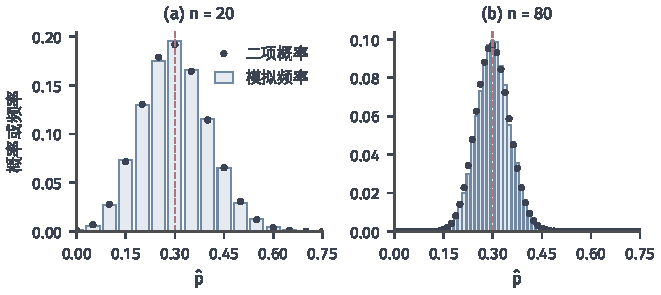
\includegraphics[width=112mm]{figures/01-basic-mathematics/05-probability-and-statistics-basics/matplotlib/samp-sample-proportion/figure.pdf}
  \caption{总体为$\operatorname{Bernoulli}(0.3)$时样本比例$\hat p$的抽样分布。每个面板用固定随机种子重复抽样$10000$次，柱高为$\hat p$各取值出现的频率，圆点为二项分布给出的精确概率，虚线标出真值$0.3$。$n=20$与$n=80$时模拟标准差分别约为$0.102$与$0.051$。}
  \label{fig:samp-sample-proportion}
\end{figure}

\paragraph{抽样分布的定义}
上面的做法对任何统计量都适用。
固定总体分布与样本量$n$后，样本$X_1,\dots,X_n$的联合分布就确定了；统计量$T=t(X_1,\dots,X_n)$是样本的函数，它的分布也随之确定。

\begin{definition}[抽样分布]
\label{def:samp-sampling-distribution}
设样本$X_1,\dots,X_n$来自给定的总体分布，$T=t(X_1,\dots,X_n)$是统计量。
把$T$作为随机变量时的概率分布称为$T$的\term{抽样分布}（sampling distribution）。
\end{definition}

抽样分布依赖三样东西：总体分布、样本量和统计量的计算规则。
总体参数未知时，抽样分布通常也含未知参数；例如$\hat p$的分布依赖$p$。
所以我们往往不能直接画出它，而是研究它的均值、方差或近似形状随参数怎样变化，这正是本章后续各节的任务。

\paragraph{三种分布的区分}
统计中经常同时出现三种“分布”，它们描述的对象不同，混淆会导致错误的结论。
\emph{总体分布}描述单个观测$X_i$的取值规律，例如一件产品是否不合格、一次测量落在哪里；它通常含未知参数。
\emph{经验分布}由一组已经得到的观测构成，第~\ref{sec:est-empirical-cdf}节用经验分布函数$\hat F_n$描述它：每个观测值占$1/n$的质量。
\emph{抽样分布}描述统计量在重复抽样中的取值规律，它的对象既不是单个观测，也不是当前这组数据。

图~\ref{fig:samp-three-distributions}用指数总体把三者放在一起。
左图是总体密度$f(x)=e^{-x}$，单个观测的波动很大，并且明显右偏。
中图是一组$n=25$的观测：经验分布函数是一条阶梯，它围绕总体分布函数随机起伏，这组数据的均值约为$1.15$。
右图把这一步重复$10000$次，统计每次的样本均值：这些均值集中在$1$附近，标准差约为$0.2$，形状也比总体对称得多。
同一个总体、同一个样本量，三幅图回答的问题完全不同。

\begin{figure*}[htbp]
  \centering
  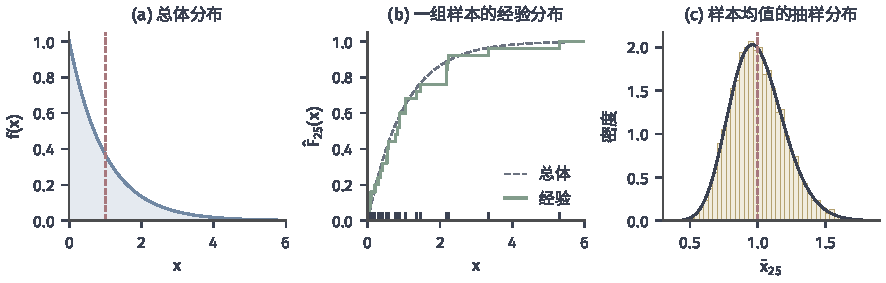
\includegraphics[width=150mm]{figures/01-basic-mathematics/05-probability-and-statistics-basics/matplotlib/samp-three-distributions/figure.pdf}
  \caption{总体分布、经验分布与抽样分布的对照。总体为率参数$1$的指数分布，均值为$1$（虚线）。(a) 总体密度；(b) 一组$n=25$观测的经验分布函数（实线阶梯）与总体分布函数（虚线），底部短线为各观测值；(c) 用固定随机种子重复抽样$10000$次得到的样本均值直方图，实线为其精确密度，即形状$25$、率$25$的Gamma分布。}
  \label{fig:samp-three-distributions}
\end{figure*}

\subsection{标准误}
\label{sec:samp-standard-error}

\paragraph{标准误的定义}
图~\ref{fig:samp-sample-proportion}中两个分布的宽度不同，我们需要一个数来概括“重复抽样时估计值的波动”。
最直接的选择是抽样分布的标准差。

\begin{definition}[标准误]
\label{def:samp-standard-error}
设统计量$T$的方差有限。$T$的抽样分布的标准差$\operatorname{SE}(T)=\sqrt{\operatorname{Var}T}$称为$T$的\term{标准误}（standard error）。
\end{definition}

标准误衡量的是计算规则的稳定性：若用同一规则在许多组独立样本上反复计算，结果大约在其均值附近$\operatorname{SE}(T)$的范围内波动。
它不说明某一次估计值离真值多远，因为单次结果仍可能落在分布的尾部；
它也不包含系统偏离，若$T$的平均位置本身就偏离目标，标准误再小也不能发现，系统偏离要由下一小节的偏差来度量。

\paragraph{样本均值的标准误}
设$X_1,\dots,X_n$独立同分布，均值$\mu$、方差$\sigma^2$有限。
由期望的线性性，$\mathbb{E}\bar X_n=\mu$。
由第~\ref{sec:rvec-moments}节，独立随机变量和的方差等于方差之和，于是
\[
  \operatorname{Var}\bar X_n=\frac1{n^2}\operatorname{Var}\Bigl(\sum_{i=1}^nX_i\Bigr)=\frac1{n^2}\sum_{i=1}^n\operatorname{Var}X_i=\frac{\sigma^2}{n},
\]
从而
\begin{equation}
  \operatorname{SE}(\bar X_n)=\frac{\sigma}{\sqrt n}.
  \label{eq:samp-mean-standard-error}
\end{equation}
这里用到独立性使交叉协方差为零；只假定同分布而观测之间正相关时，均值的方差会更大。
式~\eqref{eq:samp-mean-standard-error}说明误差以$1/\sqrt n$的速度缩小：样本量变为四倍，标准误才减半。
对样本比例，$\sigma^2=p(1-p)$，所以$\operatorname{SE}(\hat p)=\sqrt{p(1-p)/n}$；$p=0.3$时$n=20$与$n=80$分别给出$0.102$与$0.051$，与图~\ref{fig:samp-sample-proportion}的模拟值一致。

\paragraph{数据标准差与均值标准误}
$\sigma$与$\sigma/\sqrt n$描述两个不同对象的波动，不能互相替代。

\begin{example}[称重数据的两种标准差]
\label{ex:samp-weighing-standard-error}
某袋装食品的单袋净重标准差为$\sigma=10$克，随机称量$n=25$袋。
单袋净重的波动约为$10$克，这是数据的标准差，它描述袋与袋之间的差别，不会因为多称几袋而变小。
$25$袋平均净重的标准误是$10/\sqrt{25}=2$克，它描述“若重新抽取$25$袋，平均值会变化多少”，样本量越大越小。
若要把标准误降到$1$克，需要$n=(10/1)^2=100$袋。
\end{example}

实际中$\sigma$通常未知。把样本标准差$S_n$代入，得到\emph{标准误估计}$S_n/\sqrt n$；对比例则常把$\hat p$代入$\sqrt{p(1-p)/n}$。
章首检查$80$件、发现$24$件不合格的例子中，$\hat p=0.3$，标准误估计为$\sqrt{0.3\times0.7/80}\approx0.051$，它告诉读者“若重新检查$80$件，比例大约会在$\pm0.05$的量级上变动”。
标准误估计本身是一个随机量，用它代替$\sigma/\sqrt n$会带来额外误差，第~\ref{sec:samp-t}节和第~\ref{sec:samp-clt}节将分别在正态模型与大样本条件下处理这种替换。

\subsection{偏差}

\paragraph{偏差与无偏性}
标准误只看估计量围绕自身均值的波动。
我们还关心这个均值是否就是要估计的目标：如果一台秤每次都多称$3$克，读数再稳定也不准。
下面用$\mathbb{E}_\theta$表示参数取$\theta$时按样本的联合分布计算期望，以强调期望依赖未知参数。

\begin{definition}[偏差与无偏估计量]
\label{def:samp-bias}
设$\hat\theta$是参数$\theta$的估计量，且对每个$\theta\in\Theta$，$\mathbb{E}_\theta\hat\theta$存在。称
\[
  \operatorname{Bias}_\theta(\hat\theta)=\mathbb{E}_\theta\hat\theta-\theta
\]
为$\hat\theta$在$\theta$处的\term{偏差}（bias）。若对所有$\theta\in\Theta$都有$\operatorname{Bias}_\theta(\hat\theta)=0$，称$\hat\theta$为$\theta$的\term{无偏估计量}（unbiased estimator）。
\end{definition}

无偏性要求对\emph{每一个}可能的参数值都成立，因为我们事先不知道真值是哪一个；只在某个特定$\theta$处偏差为零不算无偏。
无偏性也只说明抽样分布的中心对准目标，不说明单次结果接近真值。
例如只用第一个观测$X_1$估计均值$\mu$，它满足$\mathbb{E}X_1=\mu$，是无偏的，但它的标准误是$\sigma$，不随样本量减小，用$n$个观测时仍然只利用了一个。

\paragraph{样本均值与两种方差估计}
第~\ref{chap:sample-estimation}章已经计算过几个常用统计量的期望，现在把它们放到偏差的框架中。
设$X_1,\dots,X_n$独立同分布，均值$\mu$，方差$\sigma^2$有限，$n\geq2$。

样本均值满足$\mathbb{E}\bar X_n=\mu$，因此是$\mu$的无偏估计量。

对方差，第~\ref{sec:est-sample-variance}节由平方和分解
$\sum_i(X_i-\bar X_n)^2=\sum_i(X_i-\mu)^2-n(\bar X_n-\mu)^2$
求得$\mathbb{E}\sum_i(X_i-\bar X_n)^2=n\sigma^2-\sigma^2=(n-1)\sigma^2$。
于是修正样本方差$S_n^2$满足$\mathbb{E}S_n^2=\sigma^2$，是无偏的；
分母为$n$的$\hat\sigma_n^2=\frac{n-1}{n}S_n^2$满足
\[
  \operatorname{Bias}(\hat\sigma_n^2)=\frac{n-1}{n}\sigma^2-\sigma^2=-\frac{\sigma^2}{n},
\]
平均而言低估了方差。原因是残差$X_i-\bar X_n$以样本均值为中心，而样本均值正是使平方和最小的中心，所以残差平方和系统地小于以真实$\mu$为中心的平方和。

无偏性在非线性变换下一般不保留。样本标准差$S_n=\sqrt{S_n^2}$不是$\sigma$的无偏估计量：由
$0\leq\operatorname{Var}S_n=\mathbb{E}S_n^2-(\mathbb{E}S_n)^2=\sigma^2-(\mathbb{E}S_n)^2$
得$\mathbb{E}S_n\leq\sigma$，只要$S_n$不是常数，不等号就严格成立。

\begin{example}[均匀分布端点的估计]
\label{ex:samp-uniform-maximum-bias}
设$X_1,\dots,X_n$独立同分布于$\operatorname{U}(0,\theta)$，$\theta>0$未知。第~\ref{sec:est-moments}节的矩估计是$2\bar X_n$；最大似然估计则是样本最大值$X_{(n)}$，因为似然在$\theta<X_{(n)}$时为零，在$\theta\geq X_{(n)}$时等于随$\theta$递减的$\theta^{-n}$。
由独立性，对$0\leq x\leq\theta$，
\[
  \mathbb{P}(X_{(n)}\leq x)=\prod_{i=1}^n\mathbb{P}(X_i\leq x)=\Bigl(\frac x\theta\Bigr)^n,
\]
求导得到密度$nx^{n-1}/\theta^n$，于是
\[
  \mathbb{E}X_{(n)}=\int_0^\theta x\cdot\frac{nx^{n-1}}{\theta^n}\,\mathrm{d}x=\frac{n}{n+1}\theta,\qquad
  \operatorname{Bias}_\theta(X_{(n)})=-\frac{\theta}{n+1}.
\]
最大值总落在$\theta$以下，偏差为负是可以预期的。乘上因子得到$\frac{n+1}{n}X_{(n)}$，它是无偏的；
矩估计$2\bar X_n$也是无偏的，因为$\mathbb{E}X_i=\theta/2$。同一个参数有多个无偏估计量，下一小节将说明怎样比较它们。
\end{example}

\subsection{均方误差}
\label{sec:samp-mse}

\paragraph{定义与分解}
标准误和偏差各描述误差的一个方面。为了用一个数衡量估计值离目标总体上有多远，我们取误差平方的平均。

\begin{definition}[均方误差]
\label{def:samp-mse}
设$\mathbb{E}_\theta\hat\theta^2<\infty$。称
\[
  \operatorname{MSE}_\theta(\hat\theta)=\mathbb{E}_\theta\bigl[(\hat\theta-\theta)^2\bigr]
\]
为$\hat\theta$在$\theta$处的\term{均方误差}（mean squared error, MSE）。
\end{definition}

在$\hat\theta-\theta$中加减$\mathbb{E}_\theta\hat\theta$，把误差拆成围绕均值的波动与均值的偏离：
\[
  \hat\theta-\theta=(\hat\theta-\mathbb{E}_\theta\hat\theta)+(\mathbb{E}_\theta\hat\theta-\theta).
\]
平方后取期望，第二项是常数，交叉项为$2(\mathbb{E}_\theta\hat\theta-\theta)\,\mathbb{E}_\theta(\hat\theta-\mathbb{E}_\theta\hat\theta)=0$，于是
\begin{equation}
  \operatorname{MSE}_\theta(\hat\theta)=\operatorname{Var}_\theta\hat\theta+\bigl(\operatorname{Bias}_\theta\hat\theta\bigr)^2.
  \label{eq:samp-mse-decomposition}
\end{equation}
式~\eqref{eq:samp-mse-decomposition}说明，均方误差同时惩罚波动和系统偏离；无偏估计量的均方误差就是方差，即标准误的平方。

\begin{example}[两个无偏估计量与一个有偏估计量]
\label{ex:samp-uniform-mse}
继续示例~\ref{ex:samp-uniform-maximum-bias}。由$\operatorname{Var}X_i=\theta^2/12$，矩估计的均方误差为
$\operatorname{Var}(2\bar X_n)=4\cdot\frac{\theta^2}{12n}=\frac{\theta^2}{3n}$。
对最大值，类似地算出$\mathbb{E}X_{(n)}^2=\frac{n}{n+2}\theta^2$，故
\[
  \operatorname{Var}X_{(n)}=\frac{n\theta^2}{n+2}-\frac{n^2\theta^2}{(n+1)^2}=\frac{n\theta^2}{(n+1)^2(n+2)}.
\]
再加上偏差的平方$\theta^2/(n+1)^2$，
\[
  \operatorname{MSE}(X_{(n)})=\frac{n\theta^2}{(n+1)^2(n+2)}+\frac{\theta^2}{(n+1)^2}=\frac{2\theta^2}{(n+1)(n+2)}.
\]
修正后的$\frac{n+1}{n}X_{(n)}$无偏，均方误差为$\frac{(n+1)^2}{n^2}\operatorname{Var}X_{(n)}=\frac{\theta^2}{n(n+2)}$。
取$n=10$，三者依次约为$0.0333\theta^2$、$0.0152\theta^2$、$0.0083\theta^2$。
两个无偏估计量的均方误差相差四倍；有偏的$X_{(n)}$也明显好于无偏的$2\bar X_n$。
\end{example}

\paragraph{收缩估计中的权衡}
上例中偏差与方差同时变化。下面的例子更直接地说明：主动引入偏差有时能换来更小的均方误差，但这种好处依赖未知参数。

设$X_1,\dots,X_n$独立同分布，均值$\mu$，方差$\sigma^2$已知。考虑把样本均值向$0$拉近的\term{收缩估计量}（shrinkage estimator）$c\bar X_n$，其中常数$0<c<1$。
它的偏差为$(c-1)\mu$，方差为$c^2\sigma^2/n$，所以
\[
  \operatorname{MSE}_\mu(c\bar X_n)=\frac{c^2\sigma^2}{n}+(1-c)^2\mu^2.
\]
与$\operatorname{MSE}(\bar X_n)=\sigma^2/n$相比，第一项变小了，第二项则随$|\mu|$增大而增大。

\begin{example}[收缩估计何时更好]
\label{ex:samp-shrinkage}
取$\sigma^2=1$，$n=10$，$c=0.8$。样本均值的均方误差恒为$0.1$；收缩估计的均方误差为$0.064+0.04\mu^2$。
后者更小当且仅当$0.04\mu^2<0.036$，即$|\mu|<\sqrt{0.9}\approx0.949$。
真值靠近$0$时，收缩带来的方差下降超过偏差代价；真值远离$0$时，偏差平方迅速增长，收缩反而更差。
使均方误差最小的$c$是$\mu^2/(\mu^2+\sigma^2/n)$，它依赖未知的$\mu$，所以不能直接算出。
\end{example}

图~\ref{fig:samp-shrinkage-mse}展示了这一权衡。
左图中$\mu=0.5$，收缩估计的抽样分布更窄，但中心移到了$0.4$；右图显示两条均方误差曲线在$|\mu|\approx0.949$处相交。
没有哪一个估计量对所有参数值都更好，所以比较估计量时必须说明参数范围与误差指标；
只因为一个估计量无偏就选择它，或只因为它方差小就选择它，都没有回答“离真值有多远”这个问题。

\begin{figure}[htbp]
  \centering
  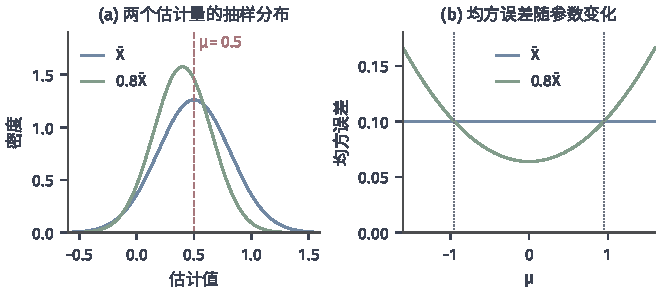
\includegraphics[width=112mm]{figures/01-basic-mathematics/05-probability-and-statistics-basics/matplotlib/samp-shrinkage-mse/figure.pdf}
  \caption{样本均值与收缩估计$0.8\bar X$的比较，总体为$\mathcal N(\mu,1)$，$n=10$。(a) $\mu=0.5$（虚线）时两个估计量的精确抽样密度：收缩估计更窄但中心偏到$0.4$。(b) 均方误差随$\mu$的变化：样本均值恒为$0.1$，收缩估计为$0.064+0.04\mu^2$，点线标出交点$|\mu|\approx0.949$。}
  \label{fig:samp-shrinkage-mse}
\end{figure}

\section{正态样本的精确抽样分布}
\label{sec:samp-normal}

上一节的误差指标只用到均值和方差。要回答“误差超过某个值的概率是多少”，需要整个抽样分布。
一般总体下这个分布很难写出；但当总体服从正态分布时，样本均值、样本方差以及由它们组成的比值都有精确的分布。
本节始终假设$X_1,\dots,X_n$独立同分布于$\mathcal N(\mu,\sigma^2)$，$n\geq2$，并把样本写成向量$\bm X=(X_1,\dots,X_n)^\top$。

\subsection{样本均值与残差}

\paragraph{常数方向上的正交分解}
记$\bm 1=(1,\dots,1)^\top\in\mathbb{R}^n$。样本均值可以写成$\bar X_n=\frac1n\bm 1^\top\bm X$，而
\[
  \bar X_n\bm 1=\frac{\bm 1\bm 1^\top}{n}\bm X
\]
恰是$\bm X$在一维子空间$\operatorname{span}\{\bm 1\}$上的正交投影：$\bm 1/\sqrt n$是该子空间的单位向量，按第~\ref{sec:ls-projection-matrices}节的投影矩阵公式，投影矩阵为$\frac{\bm 1}{\sqrt n}\frac{\bm 1^\top}{\sqrt n}=\bm 1\bm 1^\top/n$。
相应的残差向量$\bm R=\bm X-\bar X_n\bm 1$的分量是$X_i-\bar X_n$，它与$\bm 1$正交，即$\sum_iR_i=0$。
由勾股定理，
\begin{equation}
  \lVert\bm X\rVert_2^2=n\bar X_n^2+\sum_{i=1}^n(X_i-\bar X_n)^2.
  \label{eq:samp-mean-residual-pythagoras}
\end{equation}

两部分记录的信息不同。投影$\bar X_n\bm 1$只告诉我们数据的整体位置，把每个观测都换成同一个数；
残差告诉我们各观测相对这个位置怎样散开，它的平方长度除以$n-1$就是$S_n^2$。
残差受一个线性约束$\sum_iR_i=0$，所以落在$n-1$维的子空间$\{\bm r:\sum_ir_i=0\}$中，这将是后面“$n-1$个自由度”的来源。

\begin{example}[三个观测的分解]
\label{ex:samp-three-point-decomposition}
取一组观测$\bm x=(1,2,6)^\top$。样本均值为$3$，投影为$(3,3,3)^\top$，残差为$(-2,-1,3)^\top$，其分量和为$0$。
式~\eqref{eq:samp-mean-residual-pythagoras}两边分别为$1+4+36=41$与$3\cdot3^2+(4+1+9)=27+14$，相等。
修正样本方差为$14/2=7$。图~\ref{fig:samp-mean-residual-projection}按这组数据的长度画出了分解：横轴代表常数方向，纵轴代表残差所在的子空间。
\end{example}

\begin{figure}[htbp]
  \centering
  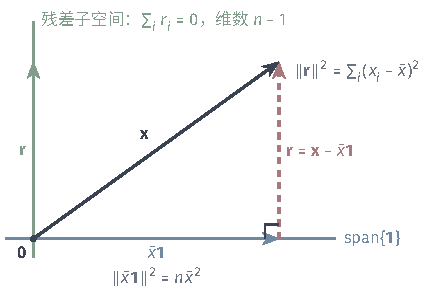
\includegraphics[width=73mm]{figures/01-basic-mathematics/05-probability-and-statistics-basics/tikz/samp-mean-residual-projection/figure.pdf}
  \caption{样本向量的正交分解示意。横轴表示一维常数方向$\operatorname{span}\{\bm 1\}$，纵轴表示$n-1$维残差子空间$\{\bm r:\sum_ir_i=0\}$。样本向量$\bm x$分解为投影$\bar x\bm 1$与残差$\bm r$，两者正交；图中长度取自$\bm x=(1,2,6)^\top$，即$\lVert\bar x\bm 1\rVert^2=27$、$\lVert\bm r\rVert^2=14$。}
  \label{fig:samp-mean-residual-projection}
\end{figure}

\paragraph{零协方差与独立性}
几何上正交并不等于概率上独立。我们先计算两部分的协方差。
由于$\operatorname{Cov}(\bar X_n,X_i)=\frac1n\sum_j\operatorname{Cov}(X_j,X_i)=\frac{\sigma^2}{n}$，
\[
  \operatorname{Cov}(\bar X_n,\,X_i-\bar X_n)=\frac{\sigma^2}{n}-\operatorname{Var}\bar X_n=\frac{\sigma^2}{n}-\frac{\sigma^2}{n}=0,\qquad i=1,\dots,n.
\]
这一计算只用到独立同分布和有限方差，对任何总体都成立。
在正态模型中，$(\bar X_n,\bm R)$是正态向量$\bm X$的线性像，因而联合高斯；第~\ref{sec:rvec-gaussian}节说明，联合高斯的两组分量交叉协方差为零时相互独立。
不过$\bm R$的协方差矩阵是奇异的（它只在$n-1$维子空间中取值），为了只使用非退化的情形，我们换一组正交坐标完成证明。

\begin{theorem}[正态样本的均值与残差]
\label{thm:samp-normal-mean-residual}
设$X_1,\dots,X_n$独立同分布于$\mathcal N(\mu,\sigma^2)$，$n\geq2$。则$\bar X_n\sim\mathcal N(\mu,\sigma^2/n)$，且$\bar X_n$与残差向量$\bm R=\bm X-\bar X_n\bm 1$相互独立。
特别地，$\bar X_n$与$S_n^2=\lVert\bm R\rVert_2^2/(n-1)$相互独立。
\end{theorem}

\begin{proof}
令$Z_i=(X_i-\mu)/\sigma$，则$Z_1,\dots,Z_n$独立同分布于$\mathcal N(0,1)$，$\bm Z$的联合密度为$(2\pi)^{-n/2}e^{-\lVert\bm z\rVert_2^2/2}$。

取$\bm q_1=\bm 1/\sqrt n$，用Gram--Schmidt正交化（定理~\ref{thm:ls-gram-schmidt}）把它扩充为$\mathbb{R}^n$的标准正交基$\bm q_1,\dots,\bm q_n$，以$\bm q_j^\top$为第$j$行组成正交矩阵$\bm Q$，并令$\bm Y=\bm Q\bm Z$。
按第~\ref{sec:rvec-transforms}节的多元变量替换，$\bm Z=\bm Q^\top\bm Y$，Jacobian行列式的绝对值为$|\det\bm Q^\top|=1$，且$\lVert\bm Q^\top\bm y\rVert_2=\lVert\bm y\rVert_2$，所以$\bm Y$的密度为
\[
  f_{\bm Y}(\bm y)=(2\pi)^{-n/2}e^{-\lVert\bm Q^\top\bm y\rVert_2^2/2}=\prod_{j=1}^n\frac1{\sqrt{2\pi}}e^{-y_j^2/2}.
\]
密度分解为乘积，说明$Y_1,\dots,Y_n$相互独立且都服从$\mathcal N(0,1)$。换一种说法：$\bm Y$联合高斯，协方差矩阵$\bm Q\bm Q^\top=\bm I$的非对角元全为零，因而各分量独立。

现在用$\bm Y$表示均值与残差。第一个坐标是
$Y_1=\bm q_1^\top\bm Z=\sqrt n\,\bar Z_n=\sqrt n(\bar X_n-\mu)/\sigma$。
由$\bm Z=\bm Q^\top\bm Y=\sum_jY_j\bm q_j$，且$Y_1\bm q_1=\bar Z_n\bm 1$，得
\[
  \bm Z-\bar Z_n\bm 1=\sum_{j=2}^nY_j\bm q_j,\qquad
  \bm R=\sigma(\bm Z-\bar Z_n\bm 1)=\sigma\sum_{j=2}^nY_j\bm q_j.
\]
于是$\bar X_n=\mu+\sigma Y_1/\sqrt n$只依赖$Y_1$，$\bm R$只依赖$(Y_2,\dots,Y_n)$。独立随机变量的两组不相交分量的函数仍相互独立（第~\ref{sec:rvec-independence}节），所以$\bar X_n$与$\bm R$独立，$S_n^2$作为$\bm R$的函数也与$\bar X_n$独立。最后$Y_1\sim\mathcal N(0,1)$给出$\bar X_n\sim\mathcal N(\mu,\sigma^2/n)$。
\end{proof}

证明中的正交矩阵$\bm Q$只是一次旋转坐标：在新坐标下，第一轴沿常数方向，其余$n-1$轴张成残差子空间。
标准正态向量的密度只依赖长度，旋转后形状不变，各坐标仍然独立；这一点是正态模型特有的。

\begin{example}[非正态总体中均值与方差不独立]
\label{ex:samp-bernoulli-mean-variance-dependent}
设$X_1,X_2$独立同分布于$\operatorname{Bernoulli}(1/2)$。此时$S_2^2=(X_1-X_2)^2/2$。
若$\bar X_2=1/2$，则$X_1\ne X_2$，$S_2^2=1/2$；若$\bar X_2\in\{0,1\}$，则$S_2^2=0$。
知道样本均值就完全确定了样本方差，两者显然不独立，尽管上面的协方差计算仍然给出$\operatorname{Cov}(\bar X_2,X_i-\bar X_2)=0$。
零协方差推出独立，依赖的是正态模型的联合高斯结构。
\end{example}

\subsection{卡方分布与样本方差}
\label{sec:samp-chi-square}

\paragraph{卡方分布的定义}
定理~\ref{thm:samp-normal-mean-residual}的证明把残差的平方长度写成了$\sigma^2\sum_{j=2}^nY_j^2$，即若干独立标准正态变量的平方和。我们先单独研究这类平方和。

\begin{definition}[卡方分布]
\label{def:samp-chi-square}
设$Z_1,\dots,Z_k$独立同分布于$\mathcal N(0,1)$，称$Q=Z_1^2+\dots+Z_k^2$的分布为自由度为$k$的\term{卡方分布}（chi-square distribution），记作$Q\sim\chi^2_k$。正整数$k$称为\term{自由度}（degrees of freedom）。
\end{definition}

自由度就是平方和中独立标准正态项的个数，也可以理解为随机向量$(Z_1,\dots,Z_k)$可以自由变化的方向数，而$Q$是它的平方长度。
由$\mathbb{E}Z_i^2=1$，$\mathbb{E}Q=k$：自由度越大，平方长度平均越大。

\paragraph{与Gamma分布的联系}
先看一项。由第~\ref{sec:prob-univariate-transforms}节平方变换的计算，$Y=Z^2$在$y>0$处的密度为两支逆像$\pm\sqrt y$的贡献之和：
\[
  f_Y(y)=\bigl(\varphi(\sqrt y)+\varphi(-\sqrt y)\bigr)\frac{1}{2\sqrt y}=\frac{1}{\sqrt{2\pi}}y^{-1/2}e^{-y/2}.
\]
与第~\ref{sec:prob-gamma}节的Gamma密度$\frac{\beta^\alpha}{\Gamma(\alpha)}y^{\alpha-1}e^{-\beta y}$比较，这正是$\operatorname{Gamma}(1/2,1/2)$，两者的常数一致也正对应$\Gamma(1/2)=\sqrt\pi$。

再看求和。设$U\sim\operatorname{Gamma}(a,\beta)$与$V\sim\operatorname{Gamma}(b,\beta)$独立，率参数相同。由卷积公式，$U+V$在$y>0$处的密度为
\[
  \int_0^y\frac{\beta^a}{\Gamma(a)}x^{a-1}e^{-\beta x}\,\frac{\beta^b}{\Gamma(b)}(y-x)^{b-1}e^{-\beta(y-x)}\,\mathrm{d}x
  =\frac{\beta^{a+b}}{\Gamma(a)\Gamma(b)}e^{-\beta y}\int_0^yx^{a-1}(y-x)^{b-1}\,\mathrm{d}x.
\]
作替换$x=yu$，最后的积分等于$y^{a+b-1}\int_0^1u^{a-1}(1-u)^{b-1}\,\mathrm{d}u$，即$y^{a+b-1}$乘以一个与$y$无关的常数。
所以$U+V$的密度正比于$y^{a+b-1}e^{-\beta y}$；密度的积分必须为$1$，比例常数只能是$\beta^{a+b}/\Gamma(a+b)$，即$U+V\sim\operatorname{Gamma}(a+b,\beta)$。
把$k$个$\operatorname{Gamma}(1/2,1/2)$逐个相加，得到
\begin{equation}
  \chi^2_k=\operatorname{Gamma}\Bigl(\frac k2,\frac12\Bigr),\qquad
  f_{\chi^2_k}(q)=\frac{1}{2^{k/2}\Gamma(k/2)}q^{k/2-1}e^{-q/2},\quad q>0.
  \label{eq:samp-chi-square-density}
\end{equation}
由Gamma分布的均值$\alpha/\beta$与方差$\alpha/\beta^2$，$\chi^2_k$的均值为$k$，方差为$2k$。

图~\ref{fig:samp-chi-square-densities}画出了几个自由度下的密度。
$k=1,2$时密度在$0$附近最大，$k\geq3$时出现内部峰值；随着$k$增大，分布中心右移到$k$附近，相对宽度$\sqrt{2k}/k$变小，形状也越来越对称。

\begin{figure}[htbp]
  \centering
  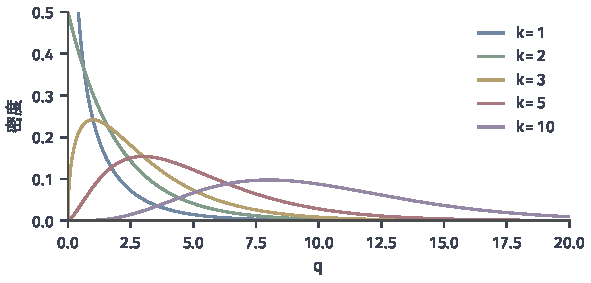
\includegraphics[width=100mm]{figures/01-basic-mathematics/05-probability-and-statistics-basics/matplotlib/samp-chi-square-densities/figure.pdf}
  \caption{自由度$k=1,2,3,5,10$的卡方分布密度，由式~\eqref{eq:samp-chi-square-density}计算。$\chi^2_k$的均值为$k$，方差为$2k$；自由度增大时分布右移、变宽，但相对其均值越来越集中且越来越对称。$k=1$时密度在$0$处趋于无穷，图中纵轴截断在$0.5$。}
  \label{fig:samp-chi-square-densities}
\end{figure}

\paragraph{样本方差的精确分布}
回到正态样本。定理~\ref{thm:samp-normal-mean-residual}的证明给出$(n-1)S_n^2=\lVert\bm R\rVert_2^2=\sigma^2\sum_{j=2}^nY_j^2$，其中$Y_2,\dots,Y_n$独立同分布于$\mathcal N(0,1)$。由定义~\ref{def:samp-chi-square}立即得到下面的结论。

\begin{theorem}[正态样本方差的分布]
\label{thm:samp-normal-sample-variance}
设$X_1,\dots,X_n$独立同分布于$\mathcal N(\mu,\sigma^2)$，$n\geq2$。则
\[
  \frac{(n-1)S_n^2}{\sigma^2}=\frac{1}{\sigma^2}\sum_{i=1}^n(X_i-\bar X_n)^2\sim\chi^2_{n-1},
\]
且它与$\bar X_n$相互独立。
\end{theorem}

自由度是$n-1$而不是$n$，原因在于残差落在$n-1$维子空间中。
如果$\mu$已知，$\sum_i(X_i-\mu)^2/\sigma^2=\sum_iZ_i^2$是$n$个独立标准正态的平方和，服从$\chi^2_n$；
改用样本均值作中心，相当于把$\bm Z$投影到与$\bm 1$正交的子空间，丢掉了沿$\bm 1$的那一个坐标$Y_1^2$。
这与第~\ref{sec:est-sample-variance}节中期望少了一个$\sigma^2$是同一现象的两种表现，只是这里得到的是完整的分布。

\begin{example}[样本方差的波动]
\label{ex:samp-sample-variance-distribution}
由定理~\ref{thm:samp-normal-sample-variance}和$\chi^2_{n-1}$的方差$2(n-1)$，
\[
  \operatorname{Var}S_n^2=\frac{\sigma^4}{(n-1)^2}\cdot2(n-1)=\frac{2\sigma^4}{n-1}.
\]
设$n=10$，$\sigma^2=4$。样本方差超过$6$的概率是$\mathbb{P}(\chi^2_9>9\cdot6/4)=\mathbb{P}(\chi^2_9>13.5)\approx0.141$：即使真实方差为$4$，也有约七分之一的机会得到大于$6$的样本方差。

这也让我们能比较两种方差估计的均方误差。$S_n^2$无偏，均方误差为$2\sigma^4/(n-1)$；
$\hat\sigma_n^2=\frac{n-1}nS_n^2$的方差为$\frac{2(n-1)\sigma^4}{n^2}$，偏差为$-\sigma^2/n$，按式~\eqref{eq:samp-mse-decomposition}，
\[
  \operatorname{MSE}(\hat\sigma_n^2)=\frac{2(n-1)\sigma^4}{n^2}+\frac{\sigma^4}{n^2}=\frac{(2n-1)\sigma^4}{n^2}.
\]
$n=10$时两者分别为$0.222\sigma^4$与$0.190\sigma^4$。在正态模型和均方误差标准下，有偏的$\hat\sigma_n^2$反而更好；这与示例~\ref{ex:samp-shrinkage}的收缩现象一致。
\end{example}

\subsection{Student $t$分布}
\label{sec:samp-t}

\paragraph{用随机标准差标准化}
若$\sigma$已知，$\sqrt n(\bar X_n-\mu)/\sigma\sim\mathcal N(0,1)$，可以直接查标准正态表。
$\sigma$未知时，自然的做法是用$S_n$代替$\sigma$，但分母因此也成了随机变量：$S_n$偶尔偏小时，比值会被放大。
我们需要一个分布描述“标准正态除以独立的随机标准差”。

\begin{definition}[$t$分布]
\label{def:samp-t}
设$Z\sim\mathcal N(0,1)$与$V\sim\chi^2_k$相互独立，称
\[
  T=\frac{Z}{\sqrt{V/k}}
\]
的分布为自由度为$k$的\term{$t$分布}（Student t distribution），记作$T\sim t_k$。
\end{definition}

分母中的$V/k$均值为$1$，是对“单位方差”的一个随机估计。
为求$T$的密度，写出$(Z,V)$的联合密度$\varphi(z)f_{\chi^2_k}(v)$，作变量替换$z=t\sqrt{v/k}$、$v=v$，Jacobian为$\sqrt{v/k}$（第~\ref{sec:rvec-transforms}节）。对$v$积分，并利用式~\eqref{eq:samp-chi-square-density}，
\[
  f_T(t)=\int_0^\infty\frac{1}{\sqrt{2\pi}}e^{-t^2v/(2k)}\sqrt{\frac vk}\cdot\frac{v^{k/2-1}e^{-v/2}}{2^{k/2}\Gamma(k/2)}\,\mathrm{d}v
  =\frac{1}{\sqrt{2\pi k}\,2^{k/2}\Gamma(k/2)}\int_0^\infty v^{\frac{k+1}2-1}e^{-\frac v2\left(1+\frac{t^2}k\right)}\,\mathrm{d}v.
\]
最后的积分是Gamma积分，等于$\Gamma\bigl(\frac{k+1}2\bigr)\bigl(\frac{2}{1+t^2/k}\bigr)^{(k+1)/2}$，化简后
\begin{equation}
  f_T(t)=\frac{\Gamma\bigl(\frac{k+1}2\bigr)}{\sqrt{k\pi}\,\Gamma\bigl(\frac k2\bigr)}\Bigl(1+\frac{t^2}{k}\Bigr)^{-(k+1)/2},\qquad t\in\mathbb{R}.
  \label{eq:samp-t-density}
\end{equation}

\paragraph{尾部与自由度}
式~\eqref{eq:samp-t-density}关于$t$对称，所以只要均值存在就等于$0$。
它的尾部按$|t|^{-(k+1)}$的幂次衰减，比正态密度的$e^{-t^2/2}$慢得多，这正是随机分母带来的额外波动。
自由度越小，尾部越重：$k=1$时$f_T(t)=\frac{1}{\pi(1+t^2)}$，即标准Cauchy分布，它的均值都不存在；一般地，$t_k$只有阶数小于$k$的矩，$k>2$时方差为$k/(k-2)$。
另一方面，$k\to\infty$时$(1+t^2/k)^{-(k+1)/2}\to e^{-t^2/2}$，$t_k$的密度逐点趋于标准正态密度，因为$V/k$越来越集中在$1$附近。

图~\ref{fig:samp-t-normal-tails}对照了几种$t$分布与标准正态。左图中$t$密度峰值更低、两侧更厚；右图用对数纵轴画双侧尾概率，差别在尾部被放大：
在$c=3$处，标准正态的尾概率约为$0.0027$，$t_{10}$约为$0.013$，$t_3$约为$0.058$，$t_1$约为$0.205$。

\begin{figure}[htbp]
  \centering
  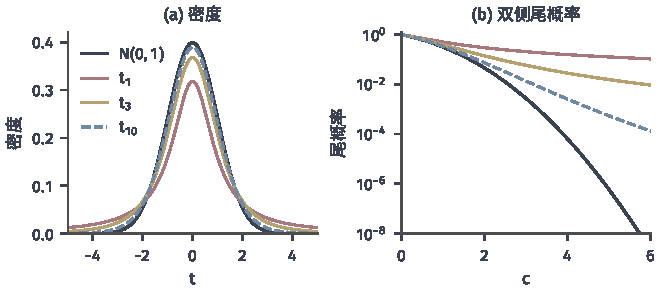
\includegraphics[width=112mm]{figures/01-basic-mathematics/05-probability-and-statistics-basics/matplotlib/samp-t-normal-tails/figure.pdf}
  \caption{Student $t$分布与标准正态分布的对照。(a) 自由度$k=1,3,10$的$t$密度与标准正态密度；(b) 双侧尾概率$\mathbb{P}(|T|>c)$，纵轴为对数刻度。自由度越小，峰越低、尾越重；$k$增大时曲线逐渐贴近标准正态。}
  \label{fig:samp-t-normal-tails}
\end{figure}

\paragraph{正态样本的$t$统计量}
定理~\ref{thm:samp-normal-mean-residual}与定理~\ref{thm:samp-normal-sample-variance}正好提供了定义~\ref{def:samp-t}所需的三个条件：
$Z=\sqrt n(\bar X_n-\mu)/\sigma\sim\mathcal N(0,1)$，$V=(n-1)S_n^2/\sigma^2\sim\chi^2_{n-1}$，且二者独立。代入定义，未知的$\sigma$恰好约去：
\begin{equation}
  T=\frac{\sqrt n(\bar X_n-\mu)}{S_n}=\frac{\sqrt n(\bar X_n-\mu)/\sigma}{\sqrt{\frac{(n-1)S_n^2/\sigma^2}{n-1}}}\sim t_{n-1}.
  \label{eq:samp-t-statistic}
\end{equation}
统计量$T$只含样本和待研究的$\mu$，它的分布不依赖任何未知参数；第~\ref{chap:intervals-tests-prediction}章将用这一点构造均值的区间与检验。

\begin{example}[用样本标准差标准化的代价]
\label{ex:samp-t-quantiles}
设$n=10$。若误把$T$当作标准正态，以为$\mathbb{P}(|T|>1.96)=0.05$，实际概率是$\mathbb{P}(|t_9|>1.96)\approx0.082$，几乎多出三分之二。
要使双侧尾概率真正为$0.05$，需要$t_{9,0.975}\approx2.262$。
下表列出不同样本量下$t_{n-1,0.975}$与$z_{0.975}\approx1.96$的比较：样本越小，用样本标准差代替$\sigma$的代价越大。
\begin{center}
\begin{tabular}{lccccc}
\toprule
$n$ & $5$ & $10$ & $30$ & $100$ & $\infty$ \\
\midrule
$t_{n-1,0.975}$ & $2.776$ & $2.262$ & $2.045$ & $1.984$ & $1.960$ \\
\bottomrule
\end{tabular}
\end{center}
\end{example}

\subsection{$F$分布}
\label{sec:samp-f}

\paragraph{两个卡方变量之比}
比较两组数据的波动时，自然的统计量是两个样本方差之比。
每个样本方差（适当缩放后）都是卡方变量，各除以自己的自由度后变成“平均每个自由度的平方长度”，再取比值。

\begin{definition}[$F$分布]
\label{def:samp-f}
设$V_1\sim\chi^2_{k_1}$与$V_2\sim\chi^2_{k_2}$相互独立，称
\[
  F=\frac{V_1/k_1}{V_2/k_2}
\]
的分布为自由度为$(k_1,k_2)$的\term{$F$分布}（F distribution），记作$F\sim F_{k_1,k_2}$。$k_1$称为分子自由度，$k_2$称为分母自由度。
\end{definition}

两个自由度分别来自分子与分母中的卡方变量，交换分子分母就交换它们：$1/F\sim F_{k_2,k_1}$。
若$T\sim t_k$，则$T^2=Z^2/(V/k)$，分子$Z^2\sim\chi^2_1$，所以$T^2\sim F_{1,k}$，$t$分布与$F$分布由此相连。
仿照$t$密度的推导，对$(V_1,V_2)$作变量替换并对辅助变量积分，可以得到$r>0$处的密度
\[
  f_{F_{k_1,k_2}}(r)=\frac{1}{B\bigl(\frac{k_1}2,\frac{k_2}2\bigr)}\Bigl(\frac{k_1}{k_2}\Bigr)^{k_1/2}r^{k_1/2-1}\Bigl(1+\frac{k_1}{k_2}r\Bigr)^{-(k_1+k_2)/2},
\]
其中$B(a,b)=\int_0^1u^{a-1}(1-u)^{b-1}\,\mathrm{d}u$是第~\ref{sec:prob-beta}节的Beta积分。

\paragraph{均值与形状}
由独立性，$\mathbb{E}F=\mathbb{E}\frac{V_1}{k_1}\cdot k_2\mathbb{E}\frac1{V_2}$。第一个因子为$1$；当$k_2>2$时，利用式~\eqref{eq:samp-chi-square-density}，
\[
  \mathbb{E}\frac1{V_2}=\int_0^\infty\frac{q^{k_2/2-2}e^{-q/2}}{2^{k_2/2}\Gamma(k_2/2)}\,\mathrm{d}q=\frac{2^{k_2/2-1}\Gamma(k_2/2-1)}{2^{k_2/2}\Gamma(k_2/2)}=\frac{1}{k_2-2},
\]
所以$\mathbb{E}F=k_2/(k_2-2)$，略大于$1$。
图~\ref{fig:samp-f-densities}显示，两个自由度都较小时$F$分布右偏、尾部很长；自由度都增大时，两个“平均平方长度”都集中在$1$附近，比值也集中在$1$附近。

\begin{figure}[htbp]
  \centering
  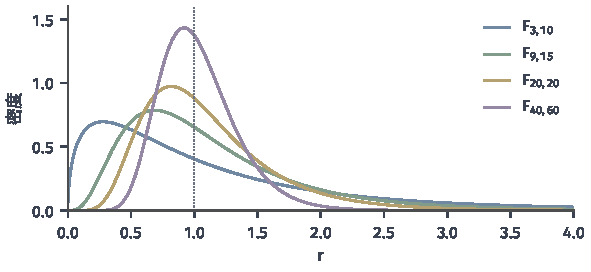
\includegraphics[width=100mm]{figures/01-basic-mathematics/05-probability-and-statistics-basics/matplotlib/samp-f-densities/figure.pdf}
  \caption{几组自由度$(k_1,k_2)$下的$F$分布密度。点线标出$r=1$。自由度小时分布右偏、尾长；两个自由度都增大时，分布向$1$附近收拢。}
  \label{fig:samp-f-densities}
\end{figure}

\paragraph{两个正态样本的方差比}
设$X_1,\dots,X_{n_1}$独立同分布于$\mathcal N(\mu_1,\sigma_1^2)$，$Y_1,\dots,Y_{n_2}$独立同分布于$\mathcal N(\mu_2,\sigma_2^2)$，两组样本相互独立，样本方差分别为$S_1^2$与$S_2^2$。
由定理~\ref{thm:samp-normal-sample-variance}，$(n_1-1)S_1^2/\sigma_1^2\sim\chi^2_{n_1-1}$，$(n_2-1)S_2^2/\sigma_2^2\sim\chi^2_{n_2-1}$，二者分别是两组独立样本的函数，因而独立。代入定义~\ref{def:samp-f}，
\begin{equation}
  \frac{S_1^2/\sigma_1^2}{S_2^2/\sigma_2^2}\sim F_{n_1-1,\,n_2-1}.
  \label{eq:samp-variance-ratio}
\end{equation}
当$\sigma_1^2=\sigma_2^2$时，未知方差约去，$S_1^2/S_2^2$本身就服从$F_{n_1-1,n_2-1}$。

\begin{example}[方差比的波动范围]
\label{ex:samp-variance-ratio}
设$n_1=10$，$n_2=16$，两总体方差相等。即使如此，$S_1^2/S_2^2\geq2.5$的概率仍为$\mathbb{P}(F_{9,15}\geq2.5)\approx0.056$；
上侧$5\%$的分界点是$F_{9,15,0.95}\approx2.59$。
所以在这样的小样本中，一个样本方差是另一个的两倍多并不罕见；第~\ref{chap:intervals-tests-prediction}章的方差比较正是以式~\eqref{eq:samp-variance-ratio}作为精确依据。
需要注意，这一结论依赖两个总体都是正态的；总体尾部较重时，样本方差的波动更大，$F$分布会低估方差比的极端程度。
\end{example}

\section{有限样本的概率界}
\label{sec:samp-bounds}
\label{sec:rv-features}

上一节的精确分布依赖正态假设。很多时候我们只知道总体的均值或方差，甚至只知道观测有界，却仍然希望对一个确定的样本量说出“误差超过某个值的概率不超过多少”。
本节的两个不等式只用矩信息就能给出这种保证。它们不要求样本量足够大，代价是给出的往往只是较宽松的上界。

\subsection{Markov不等式}

\paragraph{从期望控制尾概率}
如果一个非负随机变量经常取很大的值，它的期望就不可能很小。把这一直觉定量化，就得到用期望控制尾概率的\term{Markov不等式}（Markov inequality）。

\begin{theorem}[Markov不等式]
\label{thm:samp-markov}
设$X\geq0$，$\mathbb{E}X$有限，$a>0$。则
\begin{equation}
  \mathbb{P}(X\geq a)\leq\frac{\mathbb{E}X}{a}.
  \label{eq:samp-markov-inequality}
\end{equation}
\end{theorem}

\begin{proof}
考虑事件$\{X\geq a\}$的指示变量$\mathbb{I}_{\{X\geq a\}}$。在该事件上$X\geq a=a\,\mathbb{I}_{\{X\geq a\}}$；在其补事件上$X\geq0=a\,\mathbb{I}_{\{X\geq a\}}$。所以总有$X\geq a\,\mathbb{I}_{\{X\geq a\}}$，两边取期望，
\[
  \mathbb{E}X\geq a\,\mathbb{E}\,\mathbb{I}_{\{X\geq a\}}=a\,\mathbb{P}(X\geq a).
\]
两边除以$a>0$即得结论。
\end{proof}

证明只丢掉了两部分：事件$\{X<a\}$上$X$对期望的贡献，以及事件$\{X\geq a\}$上$X$超出$a$的部分。
两部分都为零时等号成立：例如$X$只取$0$与$a$两个值，$\mathbb{P}(X=a)=\mathbb{E}X/a$。所以只知道均值时，式~\eqref{eq:samp-markov-inequality}不能再改进。

\paragraph{条件的作用}
非负性不能去掉。若$X$以各$1/2$的概率取$-10$与$10$，则$\mathbb{E}X=0$，右端为$0$，而$\mathbb{P}(X\geq10)=1/2$：负值部分把期望拉低，抵消了大取值的贡献。
阈值必须为正，否则除法无意义；当$a\leq\mathbb{E}X$时右端不小于$1$，不等式虽然成立却没有提供信息。
对于可能取负值的变量，常见做法是先作非负变换，例如考虑$|X|$或$(X-\mu)^2$，这正是下一小节的思路。

\begin{example}[指数分布的尾概率]
\label{ex:samp-markov-exponential}
设$X$服从率参数为$1$的指数分布，$\mathbb{E}X=1$。Markov不等式给出$\mathbb{P}(X\geq3)\leq1/3$，而真实值是$e^{-3}\approx0.050$，上界大了六倍多。
图~\ref{fig:samp-markov-chebyshev}(a)显示，阈值越大差距越大：上界按$1/a$缓慢下降，真实尾概率按$e^{-a}$指数下降。
Markov不等式只利用了均值，它必须对所有均值为$1$的非负分布同时成立，其中包括上面那种把质量集中在$0$与$a$两点的极端分布，所以对具体的指数分布显得保守。
\end{example}

\begin{figure}[htbp]
  \centering
  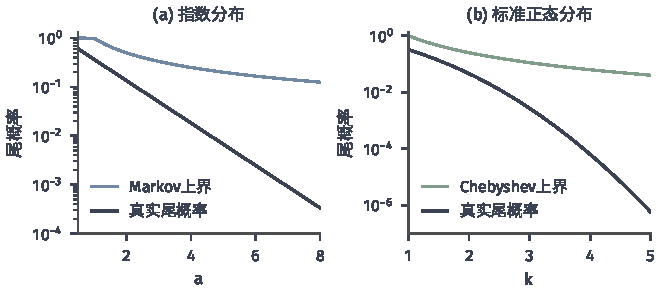
\includegraphics[width=112mm]{figures/01-basic-mathematics/05-probability-and-statistics-basics/matplotlib/samp-markov-chebyshev/figure.pdf}
  \caption{矩不等式给出的上界与真实尾概率，纵轴为对数刻度。(a) $X$服从率参数为$1$的指数分布：Markov上界$\min(1,1/a)$与真实值$\mathbb{P}(X\geq a)=e^{-a}$；(b) $Z\sim\mathcal N(0,1)$：Chebyshev上界$1/k^2$与真实值$\mathbb{P}(|Z|\geq k)$。两个上界都随阈值多项式下降，真实尾概率下降得快得多。}
  \label{fig:samp-markov-chebyshev}
\end{figure}

\subsection{Chebyshev不等式}

\paragraph{作用于平方偏离}
对一般随机变量，我们关心的是它偏离均值的程度。偏离$X-\mu$可正可负，平方解决了这个问题：$(X-\mu)^2$非负，期望恰为方差。对它使用Markov不等式，就得到\term{Chebyshev不等式}（Chebyshev inequality）。

\begin{theorem}[Chebyshev不等式]
\label{thm:samp-chebyshev}
设$X$的均值为$\mu$，方差$\sigma^2$有限。则对任意$t>0$，
\begin{equation}
  \mathbb{P}(|X-\mu|\geq t)\leq\frac{\sigma^2}{t^2}.
  \label{eq:probability-chebyshev-inequality}
\end{equation}
\end{theorem}

\begin{proof}
事件$\{|X-\mu|\geq t\}$与$\{(X-\mu)^2\geq t^2\}$相同。对非负变量$(X-\mu)^2$与阈值$t^2>0$应用Markov不等式，
\[
  \mathbb{P}(|X-\mu|\geq t)=\mathbb{P}\bigl((X-\mu)^2\geq t^2\bigr)\leq\frac{\mathbb{E}(X-\mu)^2}{t^2}=\frac{\sigma^2}{t^2}.
\]
\end{proof}

当$\sigma>0$时取$t=k\sigma$，得到更便于记忆的形式$\mathbb{P}(|X-\mu|\geq k\sigma)\leq1/k^2$：任何有限方差的分布，偏离均值两个标准差以上的概率不超过$1/4$，三个标准差以上不超过$1/9$。
和Markov不等式一样，这个界在只知道均值和方差时不能再改进：取$X$以概率$\frac1{2k^2}$分别等于$\mu\pm k\sigma$、以概率$1-\frac1{k^2}$等于$\mu$（$k\geq1$），它的方差恰为$\sigma^2$，并使等号成立。

\paragraph{与正态精确概率的对照}

\begin{example}[两个标准差与三个标准差]
\label{ex:samp-chebyshev-normal}
若$X\sim\mathcal N(\mu,\sigma^2)$，标准化后$\mathbb{P}(|X-\mu|\geq2\sigma)=2(1-\Phi(2))\approx0.046$，$\mathbb{P}(|X-\mu|\geq3\sigma)\approx0.0027$。
Chebyshev不等式给出的对应上界是$0.25$与$0.111$，分别大了约$5$倍与$40$倍。
\end{example}

这一对照说明了两类依据的区别。
正态模型给出精确概率，但只在正态假设成立时才对；Chebyshev上界对一切有限方差的分布都成立，所以必须照顾到最极端的分布，对于正态这样尾部很轻的分布就显得宽松。
图~\ref{fig:samp-markov-chebyshev}(b)把差距画在对数刻度上：上界按$1/k^2$下降，正态尾概率按$e^{-k^2/2}$量级下降。
减少分布假设与获得较紧的结论不可兼得，选择哪一种取决于我们对总体有多少可靠信息。

\subsection{样本均值误差与样本量}

\paragraph{误差、失败概率与样本量}
把Chebyshev不等式用于样本均值。设$X_1,\dots,X_n$独立同分布，均值$\mu$，方差$\sigma^2$有限。由式~\eqref{eq:samp-mean-standard-error}，$\operatorname{Var}\bar X_n=\sigma^2/n$，于是对任意$\varepsilon>0$，
\begin{equation}
  \mathbb{P}\bigl(|\bar X_n-\mu|\geq\varepsilon\bigr)\leq\frac{\sigma^2}{n\varepsilon^2}.
  \label{eq:samp-mean-chebyshev}
\end{equation}
式中出现三个量：允许的误差$\varepsilon$、误差超过$\varepsilon$的“失败概率”，以及样本量$n$。
若要求失败概率不超过$\delta\in(0,1)$，只需$\sigma^2/(n\varepsilon^2)\leq\delta$，即
\[
  n\geq\frac{\sigma^2}{\delta\varepsilon^2}.
\]
误差减半，所需样本量变为四倍；失败概率减为十分之一，所需样本量变为十倍。
例如仪器单次读数的标准差已知为$\sigma=2$，要求平均读数的误差小于$0.5$的概率至少为$0.9$，即$\varepsilon=0.5$、$\delta=0.1$，则$n\geq4/(0.1\times0.25)=160$次重复测量足以保证，且不需要知道读数服从什么分布。

\paragraph{Bernoulli均值的样本量设计}
对比例$p$，$\sigma^2=p(1-p)$依赖未知的$p$。但$p(1-p)=\frac14-(p-\frac12)^2\leq\frac14$，用这个上界代替$\sigma^2$，得到对所有$p$都有效的设计。

\begin{example}[估计支持率需要多少样本]
\label{ex:samp-chebyshev-sample-size}
希望样本比例与真实比例之差小于$0.05$的概率至少为$0.95$，即$\varepsilon=0.05$，$\delta=0.05$。由$p(1-p)\leq1/4$，
\[
  n\geq\frac{1/4}{0.05\cdot0.05^2}=2000
\]
就足够，无论$p$是多少。
这个数字偏保守。$p=1/2$时可以用二项分布直接计算失败概率：图~\ref{fig:samp-chebyshev-sample-size}显示，从$n=401$起精确失败概率就都不超过$0.05$了，只有Chebyshev要求的五分之一左右。
差距的来源与示例~\ref{ex:samp-chebyshev-normal}相同：式~\eqref{eq:samp-mean-chebyshev}只用了方差。
\end{example}

\begin{figure}[htbp]
  \centering
  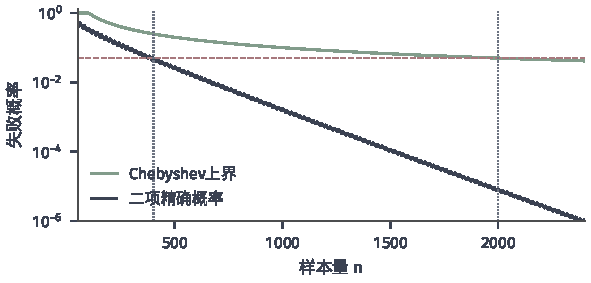
\includegraphics[width=100mm]{figures/01-basic-mathematics/05-probability-and-statistics-basics/matplotlib/samp-chebyshev-sample-size/figure.pdf}
  \caption{样本比例的失败概率$\mathbb{P}(|\hat p-0.5|\geq0.05)$随样本量$n$的变化，总体为$\operatorname{Bernoulli}(0.5)$，纵轴为对数刻度。Chebyshev上界为$100/n$，在$n=2000$处降到$0.05$（虚线）；二项分布精确概率从$n=401$起不超过$0.05$。精确曲线的锯齿来自样本比例只能取离散值。}
  \label{fig:samp-chebyshev-sample-size}
\end{figure}

\paragraph{不能直接代入样本方差}
若总体方差未知，人们容易想到先抽样算出$S_n^2$，再把它代入$\sigma^2/(n\varepsilon^2)$。
这样做得到的数是随机的，式~\eqref{eq:samp-mean-chebyshev}的证明却要求右端是确定的$\sigma^2$：
当这次样本恰好低估了方差时，计算出的“上界”偏小，而这类样本出现的概率并没有被控制，原来的严格保证因此不再成立。
要保留严格保证，需要一个预先可靠的方差上界（如比例问题中的$1/4$，或观测有界时由取值范围给出的上界）；
否则只能借助正态模型下的$t$分布或大样本下的近似，第~\ref{sec:samp-clt}节将说明后者的依据。

\section{大数定律与估计的一致性}
\label{sec:samp-lln}

式~\eqref{eq:samp-mean-chebyshev}的右端随$n\to\infty$趋于零，说明样本量增大时，样本均值偏离总体均值的概率越来越小。
本节先给这种“随机误差趋于零”的方式命名，再证明弱大数定律，最后把它用于估计量，得到一致性。

\subsection{依概率收敛}

\paragraph{定义}
对随机变量序列，“误差趋于零”可以有多种含义。我们这里采用最直接的一种：对任意固定的容许误差，误差超过它的概率趋于零。

\begin{definition}[依概率收敛]
\label{def:samp-convergence-in-probability}
设$Y_1,Y_2,\dots$与$Y$是同一随机试验中的随机变量。若对任意$\varepsilon>0$，
\[
  \lim_{n\to\infty}\mathbb{P}\bigl(|Y_n-Y|\geq\varepsilon\bigr)=0,
\]
称$Y_n$\term{依概率收敛}（convergence in probability）于$Y$，记作$Y_n\xrightarrow{\mathbb{P}}Y$。
\end{definition}

本章用到的极限$Y$几乎都是常数$c$，此时定义只涉及每个$Y_n$自己的分布：$\mathbb{P}(|Y_n-c|\geq\varepsilon)\to0$。
这里的极限是第~\ref{sec:ru-sequence-limits}节意义下的数列极限，对象是数列$a_n=\mathbb{P}(|Y_n-c|\geq\varepsilon)$；$\varepsilon$越小，通常需要越大的$n$才能使$a_n$变小。
由式~\eqref{eq:samp-mean-chebyshev}，在有限方差下$\bar X_n\xrightarrow{\mathbb{P}}\mu$，这就是下一小节的第一个定理。

\paragraph{它不保证什么}
依概率收敛描述的是每个固定$n$下误差分布的集中程度，它不要求误差随$n$单调减小。
图~\ref{fig:samp-running-means}(a)中的每一条路径都是同一组观测逐个累加时样本均值的变化：路径在前几十步内大幅上下摆动，偶尔还会离开阴影带；
但对每个固定的大$n$，绝大多数路径都已落在带内。

依概率收敛也不等于“沿着每一条观测序列，数值序列都收敛”。下面这个例子中，每个固定$n$处出错的概率都趋于零，但没有任何一条路径收敛。

\begin{example}[出错概率趋于零而路径不收敛]
\label{ex:samp-typewriter}
设$U\sim\operatorname{U}(0,1)$。把区间$[0,1)$依次分成$1$段、$2$段、$3$段……，每一轮把各段从左到右排成序列：
$[0,1)$，$[0,\tfrac12)$，$[\tfrac12,1)$，$[0,\tfrac13)$，$[\tfrac13,\tfrac23)$，$[\tfrac23,1)$，……，第$n$段记作$I_n$，令$Y_n=\mathbb{I}_{\{U\in I_n\}}$。
若$I_n$属于分成$k$段的那一轮，则$\mathbb{P}(Y_n\ne0)=1/k$，而$k\to\infty$，所以$Y_n\xrightarrow{\mathbb{P}}0$。
但对任意取定的$u\in[0,1)$，每一轮恰有一段包含$u$，所以数列$Y_n(u)$中有无穷多个$1$，也有无穷多个$0$，并不收敛。
\end{example}

沿路径的收敛是更强的要求，它属于随机变量收敛的一般理论，留到\BookPartRef{part:probability-spaces}{卷2《数学准备：抽象数学》的“概率空间”部分}。本部分只需要依概率收敛。

\subsection{弱大数定律}

\paragraph{有限方差的情形}

\begin{theorem}[弱大数定律：有限方差]
\label{thm:samp-wlln-variance}
设$X_1,X_2,\dots$独立同分布，均值$\mu$，方差$\sigma^2$有限。则$\bar X_n\xrightarrow{\mathbb{P}}\mu$。
\end{theorem}

\begin{proof}
对任意$\varepsilon>0$，由式~\eqref{eq:samp-mean-chebyshev}，$0\leq\mathbb{P}(|\bar X_n-\mu|\geq\varepsilon)\leq\sigma^2/(n\varepsilon^2)$，右端随$n\to\infty$趋于零。
\end{proof}

这个定理通常称为\term{弱大数定律}（weak law of large numbers）。“弱”指结论是依概率收敛，而不是沿路径的收敛。
它最早的形式针对事件频率。

\begin{example}[频率趋于概率]
\label{ex:samp-frequency-lln}
重复做独立试验，事件$A$每次发生的概率为$p$。令$X_i=\mathbb{I}_{\{\text{第}i\text{次试验中}A\text{发生}\}}$，则$X_i\sim\operatorname{Bernoulli}(p)$，$\bar X_n$就是前$n$次试验中$A$发生的频率。
由定理~\ref{thm:samp-wlln-variance}，频率依概率收敛于$p$；并且$\mathbb{P}(|\bar X_n-p|\geq\varepsilon)\leq p(1-p)/(n\varepsilon^2)\leq1/(4n\varepsilon^2)$。
图~\ref{fig:samp-running-means}(a)取$p=0.3$画出了六条频率路径，到$n=5000$时它们都落在$0.30\pm0.013$之内。
\end{example}

\begin{figure}[htbp]
  \centering
  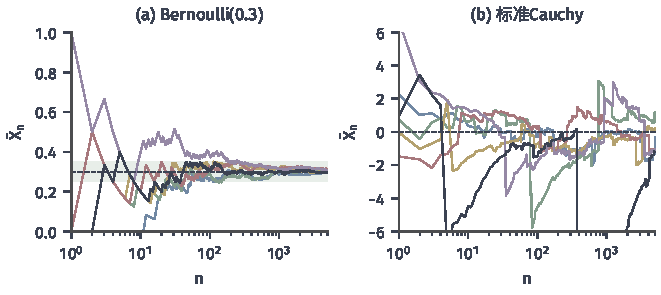
\includegraphics[width=112mm]{figures/01-basic-mathematics/05-probability-and-statistics-basics/matplotlib/samp-running-means/figure.pdf}
  \caption{样本均值$\bar X_n$随样本量$n$的变化，横轴为对数刻度，每个面板用固定随机种子画出六条独立路径。(a) 总体为$\operatorname{Bernoulli}(0.3)$，阴影带为$0.3\pm0.05$，各路径逐渐进入并停留在带内；(b) 总体为标准Cauchy分布，它没有均值，路径不断出现大跳跃，没有稳定下来的趋势（纵轴截断在$\pm6$）。}
  \label{fig:samp-running-means}
\end{figure}

\paragraph{只有一阶绝对矩的情形}
定理~\ref{thm:samp-wlln-variance}要求方差有限。但结论本身只涉及均值，我们希望在只假设$\mathbb{E}|X|<\infty$时也能得到它。
这不只是为了推广而推广：第~\ref{sec:samp-consistency}节要对$X_i^2$使用大数定律来研究样本方差，若仍要求$X_i^2$的方差有限，就需要$\mathbb{E}X^4<\infty$，比我们想要的“$X$方差有限”强得多。
另一方面，也不能完全不要矩条件：图~\ref{fig:samp-running-means}(b)中的标准Cauchy分布没有均值，可以证明它的样本均值对每个$n$都仍服从标准Cauchy分布，不会集中到任何数附近；证明需要特征函数等工具，本部分不展开。

没有方差时，Chebyshev不等式不能直接使用。思路是把每个观测分成两部分：绝对值不超过$M$的有界部分有方差，可以用Chebyshev；超过$M$的尾部方差可能不存在，但它的一阶绝对矩可以通过选大$M$变得很小，再用Markov控制。

\begin{theorem}[弱大数定律：有限一阶绝对矩]
\label{thm:samp-wlln-first-moment}
设$X_1,X_2,\dots$独立同分布，$\mathbb{E}|X_1|<\infty$，$\mu=\mathbb{E}X_1$。则$\bar X_n\xrightarrow{\mathbb{P}}\mu$。
\end{theorem}

\begin{proof}
固定$\varepsilon>0$与$\eta>0$。我们要找到$N$，使$n\geq N$时$\mathbb{P}(|\bar X_n-\mu|\geq\varepsilon)<\eta$。

\emph{第一步：截断。}对常数$M>0$，令
\[
  Y_i=X_i\,\mathbb{I}_{\{|X_i|\leq M\}},\qquad W_i=X_i\,\mathbb{I}_{\{|X_i|>M\}},
\]
则$X_i=Y_i+W_i$。$Y_1,Y_2,\dots$是各自$X_i$的函数，因而独立同分布，且$|Y_i|\leq M$；$W_i$同理。
记$\mu_M=\mathbb{E}Y_1$，$\nu_M=\mathbb{E}W_1$，则$\mu=\mu_M+\nu_M$，于是
\[
  \bar X_n-\mu=(\bar Y_n-\mu_M)+(\bar W_n-\nu_M).
\]
若$|\bar X_n-\mu|\geq\varepsilon$，两项中至少有一项的绝对值不小于$\varepsilon/2$，所以
\begin{equation}
  \mathbb{P}(|\bar X_n-\mu|\geq\varepsilon)\leq\mathbb{P}\Bigl(|\bar Y_n-\mu_M|\geq\frac\varepsilon2\Bigr)+\mathbb{P}\Bigl(|\bar W_n-\nu_M|\geq\frac\varepsilon2\Bigr).
  \label{eq:samp-truncation-split}
\end{equation}

\emph{第二步：用Markov控制尾部。}记$t_M=\mathbb{E}|W_1|=\mathbb{E}\bigl[|X_1|\,\mathbb{I}_{\{|X_1|>M\}}\bigr]$。由三角不等式与期望的线性性，
\[
  \mathbb{E}|\bar W_n-\nu_M|\leq\frac1n\sum_{i=1}^n\mathbb{E}|W_i|+|\nu_M|\leq t_M+t_M=2t_M,
\]
其中$|\nu_M|=|\mathbb{E}W_1|\leq\mathbb{E}|W_1|$。对非负变量$|\bar W_n-\nu_M|$用Markov不等式，
\[
  \mathbb{P}\Bigl(|\bar W_n-\nu_M|\geq\frac\varepsilon2\Bigr)\leq\frac{2t_M}{\varepsilon/2}=\frac{4t_M}{\varepsilon}.
\]
这个界与$n$无关。它能变小，是因为$t_M\to0$（$M\to\infty$）：在离散情形，$t_M=\sum_{|x|>M}|x|\,p_{X}(x)$是收敛级数$\sum_x|x|\,p_X(x)=\mathbb{E}|X_1|$的尾部；在有密度的情形，$t_M=\int_{|x|>M}|x|f_X(x)\,\mathrm{d}x$是收敛反常积分的尾部；两者都随$M\to\infty$趋于零。
于是可以先取定$M$，使$4t_M/\varepsilon<\eta/2$。

\emph{第三步：用Chebyshev控制有界部分。}$M$取定后，$\operatorname{Var}Y_1\leq\mathbb{E}Y_1^2\leq M^2$。由式~\eqref{eq:samp-mean-chebyshev}，
\[
  \mathbb{P}\Bigl(|\bar Y_n-\mu_M|\geq\frac\varepsilon2\Bigr)\leq\frac{M^2}{n(\varepsilon/2)^2}=\frac{4M^2}{n\varepsilon^2}.
\]
再取$N$使$4M^2/(N\varepsilon^2)<\eta/2$。代入式~\eqref{eq:samp-truncation-split}，当$n\geq N$时$\mathbb{P}(|\bar X_n-\mu|\geq\varepsilon)<\eta/2+\eta/2=\eta$。由$\eta$的任意性，结论成立。
\end{proof}

证明中两个参数的选取顺序不能颠倒。$M$越大，尾部的贡献$4t_M/\varepsilon$越小，但有界部分的上界$4M^2/(n\varepsilon^2)$越大；
若先固定$n$再选$M$，两者无法同时变小。先用$M$把尾部压到$\eta/2$以下，这一步与$n$无关；再让$n$增大去抵消已经固定的$M^2$。
截断把“没有方差”的问题化成了“有方差但方差很大”的问题，而样本量正好可以对付后者。

\subsection{估计量的一致性}
\label{sec:samp-consistency}

\paragraph{定义及与无偏性的比较}
大数定律说的是样本均值，我们把同样的要求放到一般估计量上：样本越来越多时，估计误差超过任何固定容许值的概率都趋于零。

\begin{definition}[一致性]
\label{def:samp-consistency}
设对每个样本量$n$，$\hat\theta_n$是用$X_1,\dots,X_n$构造的$\theta$的估计量。若对每个$\theta\in\Theta$，当样本按参数$\theta$生成时都有$\hat\theta_n\xrightarrow{\mathbb{P}}\theta$，称估计量序列$\{\hat\theta_n\}$具有\term{一致性}（consistency），也称它是$\theta$的一致估计量。
\end{definition}

一致性与无偏性回答的是不同的问题。无偏性固定样本量，问抽样分布的中心是否对准目标；一致性让样本量增大，问抽样分布最终是否集中到目标上。两者互不蕴含：
\begin{itemize}
  \item 只用第一个观测的$\hat\mu_n=X_1$对每个$n$都无偏，但它的分布不随$n$改变，只要$\sigma>0$就不一致。
  \item $\hat\sigma_n^2$对每个$n$都有偏，偏差$-\sigma^2/n$随$n$消失；下面会证明它是一致的。
\end{itemize}
两者之间有一个常用的联系：若$\operatorname{MSE}_\theta(\hat\theta_n)\to0$，则对$(\hat\theta_n-\theta)^2$用Markov不等式，
\[
  \mathbb{P}\bigl(|\hat\theta_n-\theta|\geq\varepsilon\bigr)\leq\frac{\operatorname{MSE}_\theta(\hat\theta_n)}{\varepsilon^2}\to0.
\]
结合式~\eqref{eq:samp-mse-decomposition}，方差与偏差都趋于零的估计量是一致的。示例~\ref{ex:samp-uniform-mse}中的三个估计量都满足这一条件。

\paragraph{依概率收敛的运算}
许多估计量是若干样本平均的连续函数。下面的引理说明，依概率收敛到常数的性质在连续函数下保持。

\begin{lemma}[连续函数保持依概率收敛]
\label{lem:samp-continuous-mapping}
设$U_n\xrightarrow{\mathbb{P}}a$，$V_n\xrightarrow{\mathbb{P}}b$，$a,b$为常数，二元函数$g$在点$(a,b)$连续。则$g(U_n,V_n)\xrightarrow{\mathbb{P}}g(a,b)$。
特别地，$U_n+V_n\xrightarrow{\mathbb{P}}a+b$，$U_nV_n\xrightarrow{\mathbb{P}}ab$；$b\neq0$时$U_n/V_n\xrightarrow{\mathbb{P}}a/b$。一元函数是其特例。
\end{lemma}

\begin{proof}
给定$\varepsilon>0$。由$g$在$(a,b)$连续，存在$\delta>0$，使$|u-a|<\delta$且$|v-b|<\delta$时$|g(u,v)-g(a,b)|<\varepsilon$。
因此事件$\{|g(U_n,V_n)-g(a,b)|\geq\varepsilon\}$包含于$\{|U_n-a|\geq\delta\}\cup\{|V_n-b|\geq\delta\}$，
\[
  \mathbb{P}\bigl(|g(U_n,V_n)-g(a,b)|\geq\varepsilon\bigr)\leq\mathbb{P}(|U_n-a|\geq\delta)+\mathbb{P}(|V_n-b|\geq\delta)\to0.
\]
比值情形中$g(u,v)=u/v$在$v=b\neq0$处连续；$V_n=0$的事件包含于$\{|V_n-b|\geq|b|\}$，其概率趋于零，不影响结论。
\end{proof}

\paragraph{样本矩与样本方差}
现在可以处理第~\ref{chap:sample-estimation}章的常用估计量。

\begin{theorem}[样本矩与样本方差的一致性]
\label{thm:samp-moment-consistency}
设$X_1,X_2,\dots$独立同分布。
\begin{enumerate}
  \item 若$\mathbb{E}|X_1|^k<\infty$，则第$k$阶样本原点矩$\frac1n\sum_{i=1}^nX_i^k\xrightarrow{\mathbb{P}}\mathbb{E}X_1^k$。
  \item 若$\mathbb{E}X_1^2<\infty$，记$\sigma^2=\operatorname{Var}X_1$，则$\hat\sigma_n^2\xrightarrow{\mathbb{P}}\sigma^2$，$S_n^2\xrightarrow{\mathbb{P}}\sigma^2$。
\end{enumerate}
\end{theorem}

\begin{proof}
(1) $X_1^k,X_2^k,\dots$独立同分布，且一阶绝对矩$\mathbb{E}|X_1^k|$有限，由定理~\ref{thm:samp-wlln-first-moment}即得。

(2) 展开平方，
\[
  \hat\sigma_n^2=\frac1n\sum_{i=1}^n(X_i-\bar X_n)^2=\frac1n\sum_{i=1}^nX_i^2-\bar X_n^2.
\]
由(1)取$k=2$与$k=1$，$\frac1n\sum_iX_i^2\xrightarrow{\mathbb{P}}\mathbb{E}X_1^2$，$\bar X_n\xrightarrow{\mathbb{P}}\mu$。对$g(u,v)=u-v^2$用引理~\ref{lem:samp-continuous-mapping}，$\hat\sigma_n^2\xrightarrow{\mathbb{P}}\mathbb{E}X_1^2-\mu^2=\sigma^2$。
最后$S_n^2=\frac{n}{n-1}\hat\sigma_n^2$，而确定的数列$\frac n{n-1}\to1$，再用一次引理即得。
\end{proof}

这里正是第~\ref{sec:samp-lln}节保留截断论证的原因：对$X_i^2$使用大数定律时，我们只知道$\mathbb{E}|X_i^2|=\mathbb{E}X_1^2<\infty$，不知道$X_i^2$的方差是否有限。

\begin{example}[矩估计的一致性]
\label{ex:samp-exponential-rate-consistency}
设$X_1,X_2,\dots$独立同分布于率参数为$\lambda$的指数分布。第~\ref{sec:est-moments}节的矩估计（也是第~\ref{sec:est-mle}节的最大似然估计）为$\hat\lambda_n=1/\bar X_n$。
由大数定律，$\bar X_n\xrightarrow{\mathbb{P}}1/\lambda>0$；函数$g(v)=1/v$在$1/\lambda$处连续，由引理~\ref{lem:samp-continuous-mapping}，$\hat\lambda_n\xrightarrow{\mathbb{P}}\lambda$。
注意$\hat\lambda_n$并不无偏：可以算出$n\geq2$时$\mathbb{E}\hat\lambda_n=\frac{n}{n-1}\lambda$。一致性不需要先算出期望。
\end{example}

\paragraph{固定阈值处的经验分布函数}
第~\ref{sec:est-empirical-cdf}节的经验分布函数在每个固定点$x$处是一个Bernoulli平均：
\[
  \hat F_n(x)=\frac1n\sum_{i=1}^n\mathbb{I}_{\{X_i\leq x\}},\qquad \mathbb{I}_{\{X_i\leq x\}}\sim\operatorname{Bernoulli}\bigl(F(x)\bigr).
\]
所以$\mathbb{E}\hat F_n(x)=F(x)$，$\operatorname{Var}\hat F_n(x)=F(x)(1-F(x))/n\leq1/(4n)$，由弱大数定律$\hat F_n(x)\xrightarrow{\mathbb{P}}F(x)$。
图~\ref{fig:samp-three-distributions}(b)中的阶梯在每个固定位置与总体曲线的差距，随样本量增大而缩小，就是这一结论。
这里的结论对每个$x$分别成立；“整条经验分布函数一致地靠近$F$”需要同时控制无穷多个点，属于更深的结果，本部分不展开。

\section{中心极限定理与正态近似}
\label{sec:samp-clt}

大数定律告诉我们$\bar X_n-\mu$依概率趋于零，却没有说明它在趋于零的过程中呈现什么形状。
要计算“误差超过$0.02$的概率约为多少”，需要把误差放大到不再消失的尺度，再研究放大后的分布。
本节说明，在有限方差的独立同分布条件下，放大后的误差近似服从正态分布，而且这个结论几乎不依赖总体的形状。

\subsection{标准化与分布收敛}

\paragraph{需要观察的对象}
由式~\eqref{eq:samp-mean-standard-error}，$\bar X_n-\mu$的标准差是$\sigma/\sqrt n$。误差按这个尺度缩小，所以要看到稳定的形状，应当除以它：
\begin{equation}
  Z_n=\frac{\bar X_n-\mu}{\sigma/\sqrt n}=\frac{\sqrt n(\bar X_n-\mu)}{\sigma}=\frac{S_n-n\mu}{\sigma\sqrt n},\qquad S_n=\sum_{i=1}^nX_i.
  \label{eq:samp-standardized-mean}
\end{equation}
这是第~\ref{sec:prob-standardization}节的标准化：对每个$n$，$\mathbb{E}Z_n=0$，$\operatorname{Var}Z_n=1$。
减去$\mu$去掉了误差的中心，除以$\sigma/\sqrt n$固定了它的尺度；剩下的问题是$Z_n$的分布形状怎样随$n$变化。
标准化本身不会让分布变成正态：$n=1$时$Z_1=(X_1-\mu)/\sigma$与总体形状相同。

\paragraph{分布收敛的定义}
$Z_n$本身并不依概率收敛到任何常数（它的方差恒为$1$），我们关心的只是它的分布是否稳定下来。
描述分布最方便的工具是分布函数。

\begin{definition}[依分布收敛]
\label{def:samp-convergence-in-distribution}
设随机变量$Y_n$的分布函数为$F_n$，$Y$的分布函数为$F$。若在$F$的每一个连续点$x$处都有$\lim_{n\to\infty}F_n(x)=F(x)$，称$Y_n$\term{依分布收敛}（convergence in distribution）于$Y$，记作$Y_n\xrightarrow{\mathrm{d}}Y$。
\end{definition}

定义只要求在$F$的连续点处收敛，是为了不让跳跃点上的取值约定影响结论。
例如$Y_n=1/n$是确定的数，自然应当“收敛到$0$”；但$F_n(0)=\mathbb{P}(1/n\leq0)=0$，而常数$0$的分布函数在$0$处等于$1$，两者在跳跃点$x=0$处不相等，其他点处都收敛。
本章的极限几乎都是标准正态分布，$\Phi$处处连续，此时定义就是对每个$x$都有$F_n(x)\to\Phi(x)$。
由此还能得到区间概率的近似：$\mathbb{P}(a<Y_n\leq b)=F_n(b)-F_n(a)\to\Phi(b)-\Phi(a)$。
把“$\leq$”换成“$<$”也不影响极限：对任意$\delta>0$有$F_n(b-\delta)\leq\mathbb{P}(Y_n<b)\leq F_n(b)$，先令$n\to\infty$再令$\delta\to0$，利用$\Phi$的连续性即可。

\paragraph{与依概率收敛的区别}
依分布收敛只比较分布，不要求$Y_n$与$Y$在同一次试验中取值接近。
例如$Z\sim\mathcal N(0,1)$，令$Y_n=-Z$对所有$n$成立。由对称性$Y_n$的分布就是$\mathcal N(0,1)$，所以$Y_n\xrightarrow{\mathrm{d}}Z$；但$|Y_n-Z|=2|Z|$不随$n$变小，$Y_n$并不依概率收敛于$Z$。
反过来，极限为常数时两者一致：$Y_n\xrightarrow{\mathbb{P}}c$意味着当$x<c$时$F_n(x)\leq\mathbb{P}(|Y_n-c|\geq c-x)\to0$，当$x>c$时$F_n(x)\geq1-\mathbb{P}(|Y_n-c|\geq x-c)\to1$，这正是在常数$c$的分布函数的连续点处收敛。

\subsection{独立同分布样本的中心极限定理}

\paragraph{定理的陈述}

\begin{theorem}[中心极限定理]
\label{thm:samp-clt}
设$X_1,X_2,\dots$独立同分布，均值$\mu$，方差$\sigma^2$满足$0<\sigma^2<\infty$。则式~\eqref{eq:samp-standardized-mean}中的$Z_n$满足$Z_n\xrightarrow{\mathrm{d}}\mathcal N(0,1)$，即对每个$x\in\mathbb{R}$，
\[
  \lim_{n\to\infty}\mathbb{P}\Bigl(\frac{\sqrt n(\bar X_n-\mu)}{\sigma}\leq x\Bigr)=\Phi(x).
\]
\end{theorem}

这一结论称为\term{中心极限定理}（central limit theorem）。它的证明需要特征函数或类似的工具来刻画分布的极限，这里不给出，一般证明见\BookPartRef{part:probability-spaces}{卷2《数学准备：抽象数学》的“概率空间”部分}。下面说明定理中每个条件和尺度的作用。

中心化$\bar X_n-\mu$使误差以$0$为中心；没有这一步，$\bar X_n$本身依概率收敛到$\mu$，谈不上形状。
方差有限且非零保证了尺度$\sigma/\sqrt n$有意义：$\sigma=0$时没有随机性，$\sigma=\infty$时不存在这样的标准化尺度。
$\sqrt n$是唯一使极限既不退化又不发散的放大倍数：若改乘$n^{a}$，$a<1/2$时放大不够，极限退化为$0$；$a>1/2$时方差$n^{2a-1}\sigma^2\to\infty$，分布向两侧散开。
最值得注意的是结论中只出现$\mu$和$\sigma$：总体是离散还是连续、是否偏斜，都不改变极限，只影响逼近的快慢。

\paragraph{用定理近似概率}
实际使用时，把“$n$足够大”理解为“$Z_n$的分布已接近$\mathcal N(0,1)$”，得到
\begin{equation}
  \mathbb{P}(S_n\leq s)=\mathbb{P}\Bigl(Z_n\leq\frac{s-n\mu}{\sigma\sqrt n}\Bigr)\approx\Phi\Bigl(\frac{s-n\mu}{\sigma\sqrt n}\Bigr).
  \label{eq:samp-clt-approximation}
\end{equation}
定理只保证$n\to\infty$时误差趋于零，并不给出某个具体$n$下误差多大；近似是否可用，需要结合第~\ref{sec:samp-normal-approximation-range}节的讨论或直接与精确值比较。

\begin{example}[二项分布的正态近似]
\label{ex:samp-de-moivre-laplace}
设$S_n\sim\operatorname{Bin}(n,p)$，看作$n$个独立$\operatorname{Bernoulli}(p)$之和，$\mu=p$，$\sigma^2=p(1-p)$。中心极限定理给出
$(S_n-np)/\sqrt{np(1-p)}\xrightarrow{\mathrm{d}}\mathcal N(0,1)$。
图~\ref{fig:samp-bernoulli-clt}取$p=0.3$，把标准化和的阶梯分布函数与$\Phi$对照：$n=10$时只有$11$个台阶，与$\Phi$的最大差距约$0.15$；$n=100$时台阶变密，最大差距约$0.05$，而且主要出现在台阶的跳跃处。
\end{example}

\begin{figure}[htbp]
  \centering
  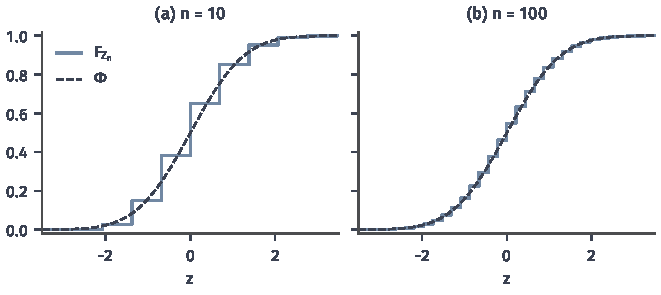
\includegraphics[width=112mm]{figures/01-basic-mathematics/05-probability-and-statistics-basics/matplotlib/samp-bernoulli-clt/figure.pdf}
  \caption{Bernoulli标准化和的分布函数与标准正态分布函数的对照。$S_n\sim\operatorname{Bin}(n,0.3)$，$Z_n=(S_n-0.3n)/\sqrt{0.21n}$；实线阶梯为$Z_n$的精确分布函数，虚线为$\Phi$。(a) $n=10$；(b) $n=100$。$n$增大时台阶变密、变低，阶梯逐渐贴近$\Phi$。}
  \label{fig:samp-bernoulli-clt}
\end{figure}

\begin{example}[平均服务时间]
\label{ex:samp-exponential-clt}
设$50$位顾客的服务时间独立同分布于率参数为$1$的指数分布（单位：分钟），$\mu=\sigma=1$。平均服务时间超过$1.2$分钟的概率约为
\[
  \mathbb{P}(\bar X_{50}>1.2)=\mathbb{P}\bigl(Z_{50}>\sqrt{50}\cdot0.2\bigr)\approx1-\Phi(1.414)\approx0.079.
\]
这里可以与精确值比较：$50\bar X_{50}$服从$\operatorname{Gamma}(50,1)$，精确概率约为$0.084$。指数分布明显右偏，$n=50$时近似已有用，但右尾仍被低估了一点。
\end{example}

\subsection{未知方差下的标准化}

\paragraph{用样本标准差替代}
式~\eqref{eq:samp-standardized-mean}需要已知$\sigma$。实际中我们只能计算
\[
  T_n=\frac{\sqrt n(\bar X_n-\mu)}{S_n}=Z_n\cdot\frac{\sigma}{S_n}.
\]
由定理~\ref{thm:samp-moment-consistency}，在有限方差下$S_n^2\xrightarrow{\mathbb{P}}\sigma^2$，再由引理~\ref{lem:samp-continuous-mapping}，$S_n/\sigma\xrightarrow{\mathbb{P}}1$。
直觉上，$n$大时乘以一个几乎等于$1$的随机因子不会改变极限分布。下面用高概率事件上的夹逼把这一直觉写成证明。

\begin{theorem}[用样本标准差标准化]
\label{thm:samp-studentized-clt}
设$X_1,X_2,\dots$独立同分布，均值$\mu$，方差$0<\sigma^2<\infty$。则$T_n=\sqrt n(\bar X_n-\mu)/S_n\xrightarrow{\mathrm{d}}\mathcal N(0,1)$。
\end{theorem}

\begin{proof}
固定$x\in\mathbb{R}$与$\delta\in(0,1)$。令$A_n=\{|S_n/\sigma-1|<\delta\}$，由$S_n/\sigma\xrightarrow{\mathbb{P}}1$，$\mathbb{P}(A_n^{\mathsf c})\to0$。

在$A_n$上$S_n>0$，且$\{T_n\leq x\}=\{Z_n\leq xS_n/\sigma\}$。这时$S_n/\sigma\in(1-\delta,1+\delta)$，所以$xS_n/\sigma$落在$x(1-\delta)$与$x(1+\delta)$之间。记这两个数中较小者为$x_-$，较大者为$x_+$（$x$为负时二者的次序与$x$为正时相反），则在$A_n$上
\[
  \{Z_n\leq x_-\}\subseteq\{T_n\leq x\}\subseteq\{Z_n\leq x_+\}.
\]
把这两个包含关系分别与$A_n$取交，再计入$A_n^{\mathsf c}$的概率，得到
\[
  \mathbb{P}(Z_n\leq x_-)-\mathbb{P}(A_n^{\mathsf c})\leq\mathbb{P}(T_n\leq x)\leq\mathbb{P}(Z_n\leq x_+)+\mathbb{P}(A_n^{\mathsf c}).
\]
令$n\to\infty$，由中心极限定理与$\mathbb{P}(A_n^{\mathsf c})\to0$，$\mathbb{P}(T_n\leq x)$的所有极限点都落在$[\Phi(x_-),\Phi(x_+)]$中。
再令$\delta\to0$，$x_\pm\to x$，由$\Phi$的连续性，上下两端都趋于$\Phi(x)$。所以$\mathbb{P}(T_n\leq x)\to\Phi(x)$。
\end{proof}

证明只用到两件事：$Z_n$的极限分布函数连续，以及替换因子依概率收敛到$1$。它没有用到$\bar X_n$与$S_n$独立，这一点很重要，因为示例~\ref{ex:samp-bernoulli-mean-variance-dependent}说明一般总体下两者并不独立。
同样的夹逼论证适用于“依分布收敛的量乘以或加上依概率收敛到常数的量”，这一般形式称为\term{Slutsky定理}（Slutsky's theorem）。

\paragraph{精确结果与渐近结果}
现在同一个统计量$T_n=\sqrt n(\bar X_n-\mu)/S_n$有了两种结论，它们的条件和含义不同。
\begin{itemize}
  \item 总体为正态时，由式~\eqref{eq:samp-t-statistic}，对每个$n\geq2$都有$T_n\sim t_{n-1}$，这是精确的有限样本结论。
  \item 总体只需方差有限时，由定理~\ref{thm:samp-studentized-clt}，$T_n$的分布在$n\to\infty$时趋于$\mathcal N(0,1)$，这是渐近结论，对固定的$n$只是近似。
\end{itemize}
两者在大样本下相容：示例~\ref{ex:samp-t-quantiles}的表中$t_{n-1,0.975}$随$n$增大趋于$1.96$。
小样本时，若有理由相信总体接近正态，用$t$分布更准确；若总体明显非正态，$t$分布不再精确，正态近似又可能尚未生效，此时两个结论都需要谨慎使用。

\subsection{正态近似的适用范围}
\label{sec:samp-normal-approximation-range}

\paragraph{偏斜、尾部与离散性}
中心极限定理不说明逼近多快。影响逼近速度的主要因素有三个。

总体越偏斜，需要的样本量越大。图~\ref{fig:samp-normal-approximation-range}(a)画出了指数总体标准化均值的精确密度：$n=1$时就是平移的指数密度，在$z=-1$处有一个跳跃；$n=5$时峰偏左、右尾偏长；$n=30$时已接近正态，但仍可看出左右不对称。
这种不对称使两侧尾部的近似误差不同：$n=5$时，右尾概率$\mathbb{P}(\bar X_5>1.5)$的精确值与正态近似都约为$0.132$，几乎相同；而对称位置的左尾概率$\mathbb{P}(\bar X_5<0.5)$精确值约为$0.109$，正态近似仍给出$0.132$。正态近似总是把两侧尾部看成一样大，偏斜总体做不到这一点。

总体尾部越重，样本中偶尔出现的极端值对均值影响越大，逼近也越慢；方差无限时定理根本不适用。

总体离散时，$S_n$只取整数，分布函数是阶梯，而$\Phi$是光滑曲线，图~\ref{fig:samp-bernoulli-clt}中的误差主要就出现在台阶的跳跃处。

\begin{figure}[htbp]
  \centering
  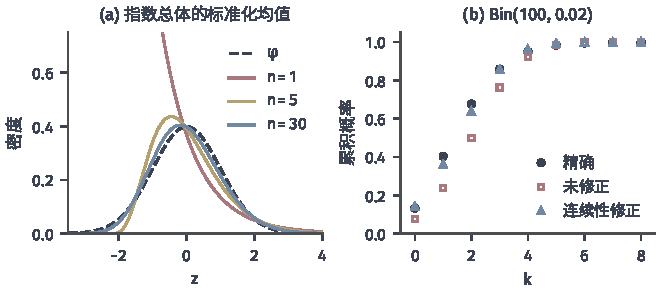
\includegraphics[width=112mm]{figures/01-basic-mathematics/05-probability-and-statistics-basics/matplotlib/samp-normal-approximation-range/figure.pdf}
  \caption{正态近似的效果取决于总体形状。(a) 率参数为$1$的指数总体下标准化均值$\sqrt n(\bar X_n-1)$的精确密度（由Gamma分布计算），$n=1,5,30$，虚线为标准正态密度$\varphi$；(b) $S\sim\operatorname{Bin}(100,0.02)$时$\mathbb{P}(S\leq k)$的精确值、未修正的正态近似与连续性修正后的近似。}
  \label{fig:samp-normal-approximation-range}
\end{figure}

\paragraph{连续性修正}
对取整数值的$S_n$，事件$\{S_n\leq k\}$与$\{S_n\leq k+\tfrac12\}$相同，与$\{S_n\leq k+0.99\}$也相同，但把它们分别代入式~\eqref{eq:samp-clt-approximation}会得到不同的近似值。
取中点$k+\tfrac12$，相当于把每个整数$j$的概率看作区间$(j-\tfrac12,j+\tfrac12]$上正态密度的面积，这称为\term{连续性修正}（continuity correction）：
\[
  \mathbb{P}(S_n\leq k)\approx\Phi\Bigl(\frac{k+\frac12-n\mu}{\sigma\sqrt n}\Bigr).
\]

\begin{example}[连续性修正的效果]
\label{ex:samp-continuity-correction}
设$S\sim\operatorname{Bin}(100,0.3)$，$np=30$，$\sqrt{np(1-p)}=\sqrt{21}\approx4.58$。精确值$\mathbb{P}(S\leq25)\approx0.163$。
不修正时近似为$\Phi\bigl((25-30)/4.58\bigr)=\Phi(-1.09)\approx0.138$；修正后为$\Phi\bigl((25.5-30)/4.58\bigr)=\Phi(-0.98)\approx0.163$，几乎与精确值相同。

再看偏斜的$S\sim\operatorname{Bin}(100,0.02)$，$np=2$，$\sqrt{np(1-p)}=1.4$。精确值$\mathbb{P}(S\geq5)=1-\mathbb{P}(S\leq4)\approx0.051$；
连续性修正后的近似为$1-\Phi\bigl((4.5-2)/1.4\bigr)\approx0.037$，不修正时为$1-\Phi\bigl((5-2)/1.4\bigr)\approx0.016$。
连续性修正改善了离散性带来的误差，却不能消除偏斜带来的误差，如图~\ref{fig:samp-normal-approximation-range}(b)所示。这时直接计算二项概率更可靠。
\end{example}

\paragraph{不能套用定理的情形}
常听到的“$n\geq30$即可用正态近似”只是经验说法，不是定理。
上例中$n=100$仍不够，因为有效的信息量取决于$np$而不是$n$；对更偏斜或尾部更重的总体，需要的样本量还会更大。
一个固定的样本量门槛不能对所有总体统一保证近似精度，使用时应检查数据的偏斜和极端值，有条件时与精确计算或模拟结果比较。

中心极限定理的两个条件也不能随意放宽。
第一，方差必须有限：标准Cauchy总体没有均值和方差，图~\ref{fig:samp-running-means}(b)中的样本均值始终不稳定，标准化更无从谈起。
第二，观测必须独立：若$X_1\sim\operatorname{Bernoulli}(1/2)$且$X_2=X_3=\dots=X_1$，则每个$\bar X_n=X_1$只取$0,1$两个值，无论$n$多大都不会接近正态。
存在依赖时，均值的方差不再是$\sigma^2/n$，有时也可以建立正态近似，但需要另外的条件，不能直接套用本节定理。

\section{本章小结}
\label{sec:samp-summary}

本章开头的问题是：按同一规则重复抽样时，估计会波动多少，样本增加后会怎样。
第一节把它落实为统计量的抽样分布，用标准误描述波动，用偏差描述系统偏离，用均方误差把两者合在一起；示例说明，无偏既不保证单次结果接近真值，也不保证均方误差最小。
其后三节给出了三类说明误差大小的依据，下表按成立条件、结果形式和所能回答的问题加以比较。

\begin{center}
\small
\begin{tabularx}{\linewidth}{>{\raggedright\arraybackslash}p{4.6em}>{\raggedright\arraybackslash}X>{\raggedright\arraybackslash}X>{\raggedright\arraybackslash}X}
\toprule
依据 & 成立条件 & 结果形式 & 能回答的问题 \\
\midrule
精确抽样分布 & 正态总体，独立同分布；样本量任意 & $\bar X_n$、$S_n^2$的分布及卡方、$t$、$F$统计量的精确分布 & 给定样本量下误差落在某范围内的确切概率 \\
有限样本概率界 & 只需均值或方差（或其上界）已知；样本量任意 & Markov、Chebyshev上界，如$\sigma^2/(n\varepsilon^2)$ & 保证失败概率不超过某值所需的样本量；结论偏保守 \\
渐近近似 & 独立同分布，方差有限；样本量趋于无穷 & 依概率收敛（大数定律、一致性）与依分布收敛（中心极限定理） & 大样本下估计是否趋于目标、误差的近似分布；有限样本精度需另行检查 \\
\bottomrule
\end{tabularx}
\end{center}

三类依据并不互相替代。精确分布最准确，但正态假设不成立时可能失效；概率界最稳健，但常常过于宽松；渐近近似适用面广且结论具体，却只在样本量足够大时可靠，而“足够大”取决于总体的偏斜、尾部和离散性。
用样本标准差代替总体标准差时，正态模型给出精确的$t$分布，一般总体则依靠一致性与Slutsky型替换得到渐近正态。

第~\ref{chap:intervals-tests-prediction}章将在这些依据上构造推断方法：正态均值与方差的区间和检验使用$t$、卡方与$F$分布；大样本的比例与均值区间使用中心极限定理和标准误估计；需要无分布假设的严格保证时，可以回到Chebyshev型的概率界。
